%%%%%%%%%%%%%%%%%%%%%%%%%%%%%%%%%%%%%%%%%%%%%%%%%%%%%%%%%%%%%%%%%%
% The following comments were written in Portuguese, because this 
% template applies only for School of Technology at University 
% of Campinas, Brazil.
%
% Este é um modelo LaTeX para monografias de Trabalhos de Conclusão 
% de Curso (TCC) na graduação da Faculdade de Engenharia Química (FEQ)
% da Universidade Estadual de Campinas (Unicamp) 
%
% Esse modelo e seu respectivo arquivo de classe de documento 
% foram adaptados do modelo de teses e dissertações do 
% Instituto de Computação e da Faculdade de Tecnologia da Unicamp, modificados incialmente por André Gradvohl. Segue o link do template original: <https://www.overleaf.com/latex/templates/template-for-graduation-work-masters-dissertation-or-doctoral-thesis-for-school-of-technology-unicamp/rhznqbkjvpcr>.
%
% Para dúvidas e sugestões, entre em contato comigo através do e-mail abaixo:
%
% Autor: Nathan Barros de Souza
% E-mail: n264179@dac.unicamp.br
% Data: 12/08/2022
%
%%%%%%%%%%%%%%%%%%%%%%%%%%%%%%%%%%%%%%%%%%%%%%%%%%%%%%%%%%%%%%%%%%

% Para a versão final do texto, acrescente a palavra "Final".
\documentclass[Portugues,Final]{TCC-FEQ}
%\documentclass[Ingles,Final]{TCC-FEQ}
%\documentclass[Espanhol,Final]{TCC-FEQ}
%
% Se o seu documento exigir uma folha de concordância da empresa, o que ocorre quando o aluno faz o TCC em algum tema do estágio, ou algum tema oferecido por uma empresa, substitua a opção "SemConcordancia" por "ComConcordancia"
%\documentclass[Portugues,Final,ComConcordancia]{TCC-FEQ}
%
% Para uma compilação mais rápida, utilize a opção "Draft", em
% letras maiúsculas como a seguir. 

%\documentclass[Portugues,Draft]{TCC-FEQ}

% Caso necessário, adicione também a opção "noFig". Essa opção 
% deixa de mostrar as figuras e, portanto, acelera mais ainda
% a compilação.
%\documentclass[Portugues,Draft,noFig]{TCC-FEQ}

%Adicione seu arquivo com as referências bibliográficas
\addbibresource{bibliografia.bib}

\usepackage{lipsum}             %O pacote a seguir gera um dummy text. Elimine a linha quando for editar seu texto.
\usepackage{float}              % Inserir figura e evitar quebra de página
\usepackage{placeins}           % Evita que um 'float' deixe uma seção
\usepackage[nopatch=footnote]{microtype}    % Melhorias de justificação
\usepackage{afterpage}          % Deixar página em branco
\usepackage{mathtools}          % Mais funcionalidade para 'amsmath'
\usepackage{nccmath}            % Ainda mais funcionalidade para 'amsmath'
\usepackage{afterpage}          % Deixar página em branco
\usepackage{xfrac}              % Para usar com \sfrac{}{}
\usepackage{csquotes}           % \begin{displayquote} - Citação direta
\usepackage{chngcntr}           % \counterwithin - Reestabelece contadores
\usepackage{systeme}            % Formatação de sistemas de equações
\usepackage{tabto}              % \tabto{} 'TAB' personalizado
\usepackage[flushleft]{threeparttable}  % Notas de tabela
\usepackage{listings}           % Para inserir códigos de program. externos
\usepackage{physics}            % Para vetores (Física)
\usepackage{xparse}             % Necessário para o pacote 'physics'
\usepackage{amsmath}            % Pacote para Matemática
\usepackage{amsthm}             % Pacote para teoremas
\usepackage{amssymb}            % Símbolos matemáticos
\usepackage{enumitem}           % Maior flexibilidade para itens e rótulos
\usepackage{textcomp}           % Mais símbolos (caracteres)
\usepackage{etoolbox}           % Interfaces LaTeX - Comandos corretivos
\usepackage{xpatch}             % Extensão para 'etoolbox'
\usepackage{multirow}           % Para tabelas extensas
\usepackage{booktabs,caption}   % Para legendas
\usepackage{tikz}               % Para criar 'checkmark'
\usepackage{icomma}             % Separador inteligente para números decimais
\usepackage{tabularx}           % Para tabelas melhores
\usepackage{nicematrix}         % Melhora a escrita de matrizes
\usepackage{hhline}             % Melhor que \hline
\usepackage{accents}            % Acentos no modo matemático
\usepackage{titlesec}           % Estilos de título
\usepackage{subfig}             % Subfigura
\usepackage{comment}            % Para comentários
\usepackage{rotating}           % Tabelas
\usepackage{pdflscape}          % Tabelas
\usepackage{changepage}
\usepackage{makecell}           % Tabelas
\usepackage{tablefootnote}      % Tabelas
\usepackage{adjustbox}          % Ajustar tabelas
\usepackage{realboxes}
\usepackage{alphalph}
\usepackage{array}
\usepackage{xstring}
\usepackage{pdfpages}

%%%%%%%%%%%%%%%%%%%%%%%%%%%%%%%%%%%%%%%%%%%%%%%%%%%%%%%%%%%%%%%%%%
% Os comandos abaixo previnem que uma figura ou tabela ('floats') 
% deixem uma determinada seção, capítulo etc.
%%%%%%%%%%%%%%%%%%%%%%%%%%%%%%%%%%%%%%%%%%%%%%%%%%%%%%%%%%%%%%%%%%
\let\Oldchapter\chapter
\renewcommand{\chapter}{\FloatBarrier\Oldchapter}

\let\Oldsection\section
\renewcommand{\section}{\FloatBarrier\Oldsection}

\let\Oldsubsection\subsection
\renewcommand{\subsection}{\FloatBarrier\Oldsubsection}

\let\Oldsubsubsection\subsubsection
\renewcommand{\subsubsection}{\FloatBarrier\Oldsubsubsection}
%%%%%%%%%%%%%%%%%%%%%%%%%%%%%%%%%%%%%%%%%%%%%%%%%%%%%%%%%%%%%%%%%%

%%%%%%%%%%%%%%%%%%%%%%%%%%%%%%%%%%%%%%%%%%%%%%%%%%%%%%%%%%%%%%%%%%
% Configurações de aparência do PDF final
%%%%%%%%%%%%%%%%%%%%%%%%%%%%%%%%%%%%%%%%%%%%%%%%%%%%%%%%%%%%%%%%%%
\definecolor{blue}{RGB}{41,5,195}   % alterando o aspecto da cor azul
\makeatletter                       % informações do PDF
\hypersetup{
		pdftitle={\@titulo},
		colorlinks=true,       		% false: boxed links; true: colored links
    	linkcolor=blue,          	% color of internal links
    	citecolor=blue,        		% color of links to bibliography
    	filecolor=magenta,      	% color of file links
		urlcolor=blue,
		bookmarksdepth=4
}
\makeatother
%%%%%%%%%%%%%%%%%%%%%%%%%%%%%%%%%%%%%%%%%%%%%%%%%%%%%%%%%%%%%%%%%%

%%%%%%%%%%%%%%%%%%%%%%%%%%%%%%%%%%%%%%%%%%%%%%%%%%%%%%%%%%%%%%%%%%
% Isto redefine funções trigonométricas para português
%%%%%%%%%%%%%%%%%%%%%%%%%%%%%%%%%%%%%%%%%%%%%%%%%%%%%%%%%%%%%%%%%%
\providecommand{\sin}{} \renewcommand{\sin}{\hspace{2pt}\mathrm{sen}}
\providecommand{\tan}{} \renewcommand{\tan}{\hspace{2pt}\mathrm{tg}}
\providecommand{\arcsin}{} \renewcommand{\arcsin}{\hspace{2pt}\mathrm{arcsen}}
%%%%%%%%%%%%%%%%%%%%%%%%%%%%%%%%%%%%%%%%%%%%%%%%%%%%%%%%%%%%%%%%%%

%%%%%%%%%%%%%%%%%%%%%%%%%%%%%%%%%%%%%%%%%%%%%%%%%%%%%%%%%%%%%%%%%%
% Isto adiciona um espaço entre o texto e a nota de rodapé.
%%%%%%%%%%%%%%%%%%%%%%%%%%%%%%%%%%%%%%%%%%%%%%%%%%%%%%%%%%%%%%%%%%
\addtolength{\skip\footins}{2pc plus 5pt}
%%%%%%%%%%%%%%%%%%%%%%%%%%%%%%%%%%%%%%%%%%%%%%%%%%%%%%%%%%%%%%%%%%

%%%%%%%%%%%%%%%%%%%%%%%%%%%%%%%%%%%%%%%%%%%%%%%%%%%%%%%%%%%%%%%%%%
% Acredito que isto faça com que páginas em branco não sejam enumeradas e não entrem na enumeração do sumário.
%%%%%%%%%%%%%%%%%%%%%%%%%%%%%%%%%%%%%%%%%%%%%%%%%%%%%%%%%%%%%%%%%%
\newcommand\blankpage{%
    \null
    \thispagestyle{empty}%
    \addtocounter{page}{-1}%
    \newpage}
%%%%%%%%%%%%%%%%%%%%%%%%%%%%%%%%%%%%%%%%%%%%%%%%%%%%%%%%%%%%%%%%%%

%%%%%%%%%%%%%%%%%%%%%%%%%%%%%%%%%%%%%%%%%%%%%%%%%%%%%%%%%%%%%%%%%%
% Isso foi necessário para remover o espaçamento que aparecia após uma equação, mas nunca antes dela. Dessa forma, o texto ficava mal formatado.
%%%%%%%%%%%%%%%%%%%%%%%%%%%%%%%%%%%%%%%%%%%%%%%%%%%%%%%%%%%%%%%%%%
\xpatchcmd{\NCC@ignorepar}{%
    \abovedisplayskip\abovedisplayshortskip}{%
    \abovedisplayskip\abovedisplayshortskip%
    \belowdisplayskip\belowdisplayshortskip}
    {}{}
%%%%%%%%%%%%%%%%%%%%%%%%%%%%%%%%%%%%%%%%%%%%%%%%%%%%%%%%%%%%%%%%%%

%%%%%%%%%%%%%%%%%%%%%%%%%%%%%%%%%%%%%%%%%%%%%%%%%%%%%%%%%%%%%%%%%%
% Corrige a quebra de linha ao utilizar o comando \texttt
%%%%%%%%%%%%%%%%%%%%%%%%%%%%%%%%%%%%%%%%%%%%%%%%%%%%%%%%%%%%%%%%%%
\let\oldtexttt\texttt
\renewcommand{\texttt}[1]{\oldtexttt{\StrSubstitute[0]{#1}{.}{.\allowbreak}}}
%%%%%%%%%%%%%%%%%%%%%%%%%%%%%%%%%%%%%%%%%%%%%%%%%%%%%%%%%%%%%%%%%%

\begin{document}

%%%%%%%%%%%%%%%%%%%%%%%%%%%%%%%%%%%%%%%%%%%%%%%%%%%%%%%%%%%%%%%%%%
% The following comments were written in Portuguese, because this 
% template applies only for School of Technology at University 
% of Campinas, Brazil.
%%%%%%%%%%%%%%%%%%%%%%%%%%%%%%%%%%%%%%%%%%%%%%%%%%%%%%%%%%%%%%%%%%
% Este é um modelo LaTeX para monografias de Trabalhos de Conclusão
% de Curso (TCC) na graduação da Faculdade de Engenharia Química 
% (FEQ) da Universidade Estadual de Campinas (Unicamp). 
%%%%%%%%%%%%%%%%%%%%%%%%%%%%%%%%%%%%%%%%%%%%%%%%%%%%%%%%%%%%%%%%%%
% Esse modelo e seu respectivo arquivo de classe de documento 
% foram adaptados do modelo de teses e dissertações do 
% Instituto de Computação e da Faculdade de Tecnologia da Unicamp, 
% modificados inicialmente por André Gradvohl. Segue o link do 
% template original com outros modelos para dissertação e teses: 
% <https://www.overleaf.com/latex/templates/template-for-graduation
% -work-masters-dissertation-or-doctoral-thesis-for-school-of-techn
% ology-unicamp/rhznqbkjvpcr>.
%%%%%%%%%%%%%%%%%%%%%%%%%%%%%%%%%%%%%%%%%%%%%%%%%%%%%%%%%%%%%%%%%%
% Para dúvidas e sugestões, entre em contato comigo através do e-mail abaixo:
%%%%%%%%%%%%%%%%%%%%%%%%%%%%%%%%%%%%%%%%%%%%%%%%%%%%%%%%%%%%%%%%%%
% Autor: Nathan Barros de Souza
% E-mail: n264179@dac.unicamp.br
% Data: 12/08/2022
%%%%%%%%%%%%%%%%%%%%%%%%%%%%%%%%%%%%%%%%%%%%%%%%%%%%%%%%%%%%%%%%%%

%%%%%%%%%%%%%%%%%%%%%%%%%%%%%%%%%%%%%%%%%%%%%%%%%%%%%%%%%%%%%%%%%%
% Antes de tudo, abra o arquivo "TCC.tex" e verifique se os 
% parâmetros do comando "\documentclass" estão de acordo com o que 
% você deseja.
%%%%%%%%%%%%%%%%%%%%%%%%%%%%%%%%%%%%%%%%%%%%%%%%%%%%%%%%%%%%%%%%%%

%%%%%%%%%%%%%%%%%%%%%%%%%%%%%%%%%%%%%%%%%%%%%%%%%%%%%%%%%%%%%%%%%%
% Escolha o número de autores (comente um e descomente o outro):
%%%%%%%%%%%%%%%%%%%%%%%%%%%%%%%%%%%%%%%%%%%%%%%%%%%%%%%%%%%%%%%%%%
\setcounter{counterauthors}{1} % Para apenas um autor
%\setcounter{counterauthors}{2} % Para dois autores
%%%%%%%%%%%%%%%%%%%%%%%%%%%%%%%%%%%%%%%%%%%%%%%%%%%%%%%%%%%%%%%%%%

%%%%%%%%%%%%%%%%%%%%%%%%%%%%%%%%%%%%%%%%%%%%%%%%%%%%%%%%%%%%%%%%%%
% Escolha entre primeiro autor ou primeira autora (comente um e 
% descomente o outro):
%%%%%%%%%%%%%%%%%%%%%%%%%%%%%%%%%%%%%%%%%%%%%%%%%%%%%%%%%%%%%%%%%%
%\primeiroautor{Nome do primeiro autor}
\primeiraautora{Débora Ferreira Deotti}
%%%%%%%%%%%%%%%%%%%%%%%%%%%%%%%%%%%%%%%%%%%%%%%%%%%%%%%%%%%%%%%%%%

%%%%%%%%%%%%%%%%%%%%%%%%%%%%%%%%%%%%%%%%%%%%%%%%%%%%%%%%%%%%%%%%%%
% Caso haja mais de um autor, escolha entre segundo autor ou 
% segunda autora (comente um e descomente o outro):
%%%%%%%%%%%%%%%%%%%%%%%%%%%%%%%%%%%%%%%%%%%%%%%%%%%%%%%%%%%%%%%%%%
% OBS.: Se não houver 2 autores, deixe ambos comentados!
%%%%%%%%%%%%%%%%%%%%%%%%%%%%%%%%%%%%%%%%%%%%%%%%%%%%%%%%%%%%%%%%%%
% Aconselha-se ordenar os autores (primeiro e segundo) em ordem 
% alfabética.
%%%%%%%%%%%%%%%%%%%%%%%%%%%%%%%%%%%%%%%%%%%%%%%%%%%%%%%%%%%%%%%%%%
%\segundoautor{Nome do segundo autor}
%\segundaautora{Nome da segunda autora}
%%%%%%%%%%%%%%%%%%%%%%%%%%%%%%%%%%%%%%%%%%%%%%%%%%%%%%%%%%%%%%%%%%

%%%%%%%%%%%%%%%%%%%%%%%%%%%%%%%%%%%%%%%%%%%%%%%%%%%%%%%%%%%%%%%%%%
% Sempre deve haver um título em português:
%%%%%%%%%%%%%%%%%%%%%%%%%%%%%%%%%%%%%%%%%%%%%%%%%%%%%%%%%%%%%%%%%%
\titulo{Modelagem Computacional da Liberação
Controlada de Etinilestradiol em Diferentes Matrizes}
%%%%%%%%%%%%%%%%%%%%%%%%%%%%%%%%%%%%%%%%%%%%%%%%%%%%%%%%%%%%%%%%%%

%%%%%%%%%%%%%%%%%%%%%%%%%%%%%%%%%%%%%%%%%%%%%%%%%%%%%%%%%%%%%%%%%%
% Se a língua for o inglês ou o espanhol, descomente:
%%%%%%%%%%%%%%%%%%%%%%%%%%%%%%%%%%%%%%%%%%%%%%%%%%%%%%%%%%%%%%%%%%
%\title{The Title in English or Spanish}
%%%%%%%%%%%%%%%%%%%%%%%%%%%%%%%%%%%%%%%%%%%%%%%%%%%%%%%%%%%%%%%%%%

%%%%%%%%%%%%%%%%%%%%%%%%%%%%%%%%%%%%%%%%%%%%%%%%%%%%%%%%%%%%%%%%%%
% Escolha entre supervisor ou supervisora e inclua os títulos 
% (comente um e descomente o outro):
%%%%%%%%%%%%%%%%%%%%%%%%%%%%%%%%%%%%%%%%%%%%%%%%%%%%%%%%%%%%%%%%%%
\supervisor{Prof. Dr. Raphael Soeiro Suppino}
%\supervisora{Profa. Dra. Nome da Supervisora}
%%%%%%%%%%%%%%%%%%%%%%%%%%%%%%%%%%%%%%%%%%%%%%%%%%%%%%%%%%%%%%%%%%

%%%%%%%%%%%%%%%%%%%%%%%%%%%%%%%%%%%%%%%%%%%%%%%%%%%%%%%%%%%%%%%%%%
% Escolha o nome da cidade e a sigla do estado em que o trabalho 
% será defendido:
%%%%%%%%%%%%%%%%%%%%%%%%%%%%%%%%%%%%%%%%%%%%%%%%%%%%%%%%%%%%%%%%%%
\cidade{Campinas}
\estadosigla{SP}
%%%%%%%%%%%%%%%%%%%%%%%%%%%%%%%%%%%%%%%%%%%%%%%%%%%%%%%%%%%%%%%%%%

%%%%%%%%%%%%%%%%%%%%%%%%%%%%%%%%%%%%%%%%%%%%%%%%%%%%%%%%%%%%%%%%%%
% Data da defesa
%%%%%%%%%%%%%%%%%%%%%%%%%%%%%%%%%%%%%%%%%%%%%%%%%%%%%%%%%%%%%%%%%%
\datadadefesa{04}{11}{2024}
%%%%%%%%%%%%%%%%%%%%%%%%%%%%%%%%%%%%%%%%%%%%%%%%%%%%%%%%%%%%%%%%%%

\inicializacao

% Tipo de modelo (TCC)
\bsi

% Este comando deve ficar aqui:
\paginasiniciais

%%%%%%%%%%%%%%%%%%%%%%%%%%%%%%%%%%%%%%%%%%%%%%%%%%%%%%%%%%%%%%%%%%
% Adicione no arquivo "preambulo_01_dedicatoria.tex" a sua 
% dedicatória.
% Se não houver dedicatória, comente a linha a seguir:
%%%%%%%%%%%%%%%%%%%%%%%%%%%%%%%%%%%%%%%%%%%%%%%%%%%%%%%%%%%%%%%%%%
% \input{preenchimento/pretextual_01_dedicatoria}
%%%%%%%%%%%%%%%%%%%%%%%%%%%%%%%%%%%%%%%%%%%%%%%%%%%%%%%%%%%%%%%%%%

%%%%%%%%%%%%%%%%%%%%%%%%%%%%%%%%%%%%%%%%%%%%%%%%%%%%%%%%%%%%%%%%%%
% Adicione no arquivo "preambulo_02_epigrafe.tex" a epígrafe
% Se não houver epígrafe, comente a linha a seguir:
%%%%%%%%%%%%%%%%%%%%%%%%%%%%%%%%%%%%%%%%%%%%%%%%%%%%%%%%%%%%%%%%%%
%\input{preenchimento/pretextual_02_epigrafe}
%%%%%%%%%%%%%%%%%%%%%%%%%%%%%%%%%%%%%%%%%%%%%%%%%%%%%%%%%%%%%%%%%%

%%%%%%%%%%%%%%%%%%%%%%%%%%%%%%%%%%%%%%%%%%%%%%%%%%%%%%%%%%%%%%%%%%
% Adicione no arquivo "preambulo_03_agradecimentos.tex" os seus 
% agradecimentos.
% Se não houver agradecimentos, comente a linha a seguir:
%%%%%%%%%%%%%%%%%%%%%%%%%%%%%%%%%%%%%%%%%%%%%%%%%%%%%%%%%%%%%%%%%%
% \input{preenchimento/pretextual_03_agradecimentos}
%%%%%%%%%%%%%%%%%%%%%%%%%%%%%%%%%%%%%%%%%%%%%%%%%%%%%%%%%%%%%%%%%%

%%%%%%%%%%%%%%%%%%%%%%%%%%%%%%%%%%%%%%%%%%%%%%%%%%%%%%%%%%%%%%%%%%
% Sempre deve haver um resumo em português:
%%%%%%%%%%%%%%%%%%%%%%%%%%%%%%%%%%%%%%%%%%%%%%%%%%%%%%%%%%%%%%%%%%
\begin{resumo}
A exclusão histórica das mulheres da pesquisa médica resultou em vieses na compreensão das questões de saúde feminina. Este trabalho visa aprimorar os conhecimentos relativos aos métodos de liberação de etinilestradiol (EE), um estrogênio sintético utilizado em diversos métodos contraceptivos. Para isso, foi realizada a modelagem matemática e computacional da liberação controlada de etinilestradiol em diferentes matrizes de liberação, especificamente o adesivo transdérmico, anel vaginal e comprimido oral combinado (COC), conhecido popularmente como pílula anticoncepcional. Cada sistema de liberação possui características próprias de difusão e liberação controlada, atendendo a necessidades específicas de administração de hormônios em contraceptivos combinados. Para o adesivo transdérmico e o anel vaginal, foi utilizado um modelo de difusão baseado em equações diferenciais parciais (EDPs) para simular o transporte de EE através das camadas da matriz. As condições de contorno pertinentes às restrições de cada sistema foram aplicadas, e as equações foram resolvidas através do método numérico de Crank-Nicolson utilizando Python. Para a pílula anticoncepcional, foi utilizada a equação de Noyes-Whitney, descrevendo a dissolução do EE no fluido gastrointestinal por meio de um modelo cinético de primeira ordem. A EDO correspondente foi resolvida utilizando o método de Runge-Kutta de quarta ordem (RK4). Foram plotados gráficos para ilustrar a difusão do EE ao longo das camadas poliméricas e sua liberação a partir de cada uma das matrizes. Os resultados indicam que o adesivo transdérmico proporciona uma liberação sustentada de EE ao longo de sete dias, enquanto o anel vaginal exibe uma liberação inicial rápida seguida de estabilização ao longo de três semanas. O COC, por sua vez, apresenta concentrações muito mais altas e flutuações significativas na liberação, necessitando de administração diária para manter níveis terapêuticos adequados. As limitações do estudo incluem a não consideração dos processos metabólicos e da resistência da pele. A análise de sensibilidade realizada para o coeficiente de difusão \( D \) revelou que variações nesse parâmetro afetam significativamente a taxa de liberação do fármaco. Valores maiores de \( D \) resultam em uma difusão mais rápida, enquanto valores menores resultam em uma difusão mais lenta, impactando diretamente o desempenho do sistema de liberação. Concluiu-se que a modelagem computacional é uma ferramenta valiosa para otimizar os mecanismos de liberação de medicamentos, melhorando a segurança e a eficácia dos métodos contraceptivos e contribuindo para melhores condições de saúde para as mulheres.
\end{resumo}
%%%%%%%%%%%%%%%%%%%%%%%%%%%%%%%%%%%%%%%%%%%%%%%%%%%%%%%%%%%%%%%%%%

%%%%%%%%%%%%%%%%%%%%%%%%%%%%%%%%%%%%%%%%%%%%%%%%%%%%%%%%%%%%%%%%%%

%%%%%%%%%%%%%%%%%%%%%%%%%%%%%%%%%%%%%%%%%%%%%%%%%%%%%%%%%%%%%%%%%%
% A lista de figuras:
%%%%%%%%%%%%%%%%%%%%%%%%%%%%%%%%%%%%%%%%%%%%%%%%%%%%%%%%%%%%%%%%%%
\listoffigures
%%%%%%%%%%%%%%%%%%%%%%%%%%%%%%%%%%%%%%%%%%%%%%%%%%%%%%%%%%%%%%%%%%

%%%%%%%%%%%%%%%%%%%%%%%%%%%%%%%%%%%%%%%%%%%%%%%%%%%%%%%%%%%%%%%%%%
% A lista de tabelas:
%%%%%%%%%%%%%%%%%%%%%%%%%%%%%%%%%%%%%%%%%%%%%%%%%%%%%%%%%%%%%%%%%%
%\listoftables
%%%%%%%%%%%%%%%%%%%%%%%%%%%%%%%%%%%%%%%%%%%%%%%%%%%%%%%%%%%%%%%%%%

%%%%%%%%%%%%%%%%%%%%%%%%%%%%%%%%%%%%%%%%%%%%%%%%%%%%%%%%%%%%%%%%%%
% A lista de símbolos é opcional. Não confunda a lista de símbolos 
% matemáticos com a lista de abreviaturas (que vem depois).
% Se não houver uma lista de símbolos, comente a linha a seguir:
%%%%%%%%%%%%%%%%%%%%%%%%%%%%%%%%%%%%%%%%%%%%%%%%%%%%%%%%%%%%%%%%%%
%\input{preenchimento/pretextual_05_listaSimbolos}
%%%%%%%%%%%%%%%%%%%%%%%%%%%%%%%%%%%%%%%%%%%%%%%%%%%%%%%%%%%%%%%%%%

%%%%%%%%%%%%%%%%%%%%%%%%%%%%%%%%%%%%%%%%%%%%%%%%%%%%%%%%%%%%%%%%%%
% A lista de abreviações e siglas vem a seguir.
% Dê uma olhada no pacote "nomencl" para ver os comandos para 
% adicionar abreviações e siglas no texto.
% Foram adicionados os comandos \Sigla{Sigla por extenso}{abrev} e 
% \SiglaHifen{Sigla por extenso}{abrev} para adicionar as siglas
% diretamente no texto e criar a lisa de abreviaturas 
% automaticamente.
%%%%%%%%%%%%%%%%%%%%%%%%%%%%%%%%%%%%%%%%%%%%%%%%%%%%%%%%%%%%%%%%%%
\printnomenclature[3cm]
%%%%%%%%%%%%%%%%%%%%%%%%%%%%%%%%%%%%%%%%%%%%%%%%%%%%%%%%%%%%%%%%%%

%%%%%%%%%%%%%%%%%%%%%%%%%%%%%%%%%%%%%%%%%%%%%%%%%%%%%%%%%%%%%%%%%%
% O sumário vem aqui:
%%%%%%%%%%%%%%%%%%%%%%%%%%%%%%%%%%%%%%%%%%%%%%%%%%%%%%%%%%%%%%%%%%
\tableofcontents
%%%%%%%%%%%%%%%%%%%%%%%%%%%%%%%%%%%%%%%%%%%%%%%%%%%%%%%%%%%%%%%%%%

% E a linha a seguir deve ficar bem aqui. Não mude.
\fimdaspaginasiniciais

%%%%%%%%%%%%%%%%%%%%%%%%%%%%%%%%%%%%%%%%%%%%%%%%%%%%%%%%%%%%%%%%%%
% O corpo da dissertação ou tese começa aqui:
%%%%%%%%%%%%%%%%%%%%%%%%%%%%%%%%%%%%%%%%%%%%%%%%%%%%%%%%%%%%%%%%%%
% O comando a seguir inclui o arquivo introducao.tex que contém o 
% capítulo de Introdução. 
%%%%%%%%%%%%%%%%%%%%%%%%%%%%%%%%%%%%%%%%%%%%%%%%%%%%%%%%%%%%%%%%%%
%%%%%%%%%%%%%%%%%%%%%%%%%%%%%%%%%%%%%%%%%%%%%%%%%%%%%%%%%%%%%%%%%%
% Aqui começa o capítulo de Introdução.
%%%%%%%%%%%%%%%%%%%%%%%%%%%%%%%%%%%%%%%%%%%%%%%%%%%%%%%%%%%%%%%%%%
% Use o comando \label para definir um rótulo, caso seja 
% necessário referenciar esse capítulo posteriormente.
%%%%%%%%%%%%%%%%%%%%%%%%%%%%%%%%%%%%%%%%%%%%%%%%%%%%%%%%%%%%%%%%%%
\chapter{Introdução}\label{chp:Introducao}
%%%%%%%%%%%%%%%%%%%%%%%%%%%%%%%%%%%%%%%%%%%%%%%%%%%%%%%%%%%%%%%%%%

\section{Contextualização}\label{sec:context}

Até o século XVIII, o pensamento médico da Europa acreditava na existência de um só sexo, o masculino. A mulher era o seu representante inferior, representada anatomicamente com o crânio menor e o quadril maior do que os do esqueleto masculino, refletindo a crença vigente de que possuiria menor capacidade intelectual e estaria naturalmente destinada somente à maternidade (Fernandes, 2009; Jackson, 2021). 

Historicamente, participantes do sexo feminino foram excluídos de estudos clínicos devido aos efeitos do ciclo menstrual aumentarem a complexidade e os custos da pesquisa e ao receio de que o tratamento investigado afetasse a fertilidade feminina ou a gravidez, além da suposta maior incidência de algumas doenças entre homens (Couto, 2021). Essa falta de inclusão perpetuada ao longo dos séculos deu origem a uma medicina com compreensão limitada da saúde feminina, o que pode levar a diagnósticos incorretos, tratamentos inadequados e negligência de sintomas ou efeitos colaterais. Porém, para além dos médicos, cientistas e pesquisadores também são majoritariamente homens, bem como a maioria das células, animais e corpos estudados na ciência são pertencentes ao sexo masculino (Jackson, 2021).

A tendência da falta de conhecimento médico e científico se torna ainda mais evidente em muitas condições predominantemente femininas. Por exemplo, mulheres com endometriose frequentemente recebem informações de que o adiamento da maternidade é a causa da doença, ou que a gravidez pode ser a cura, refletindo a antiga crença de que  a maternidade, vista como a verdadeira essência das mulheres, constituía o remédio para seus distúrbios (Fernandes, 2009). Mulheres com câncer de mama também já foram orientadas dessa mesma maneira até que avanços na pesquisa, que só ocorreram devido às campanhas realizadas por mulheres, demonstraram o contrário (Jackson, 2021).

Desde a década de 1990, houve um esforço para incluir mais mulheres nos ensaios clínicos, originado em campanhas de mulheres cientistas nos Estados Unidos que pediam por melhores pesquisas em saúde da mulher. Em resposta, em 1993 as agências governamentais norte-americanas FDA (Food and Drug Administration) e NIH (National Institutes of Health) passaram a exigir análises específicas de segurança e eficácia por sexo para todas as novas aplicações de medicamentos. Além disso, mulheres em idade fértil passaram a ser permitidas nas fases iniciais dos ensaios clínicos, removendo uma restrição significativa que anteriormente limitava a participação feminina (Jackson, 2021; Berg, 1997).  

Essa não foi a primeira vez na história recente que as mulheres influenciaram as prioridades da produção científica com relação à saúde feminina. Algumas décadas antes, a criação da primeira pílula anticoncepcional, nos anos 1960, foi resultado de uma pesquisa financiada por uma mulher feminista, a norte-americana Margaret Sanger, fundadora da Planned Parenthood Federation of America (PPFA). Na década de 40, o biólogo Gregory Pincus estudava o efeito anti-ovulatório de hormônios sexuais em animais. O impulso para converter as descobertas obtidas com seus experimentos em contracepção hormonal para humanos foi dado por Sanger, em 1951. A partir disso, Pincus passou a colaborar com John Rock, ginecologista e especialista em fertilidade, o que resultou no desenvolvimento da primeira pílula anticoncepcional, aprovada em 1960, que continha versões primitivas de progesterona e estrogênio sintéticos (Dhont, 2010). 

O estradiol, principal estrogênio humano natural, possui baixa absorção quando administrado oralmente, além de ser rapidamente inativado pelo fígado. O químico Hans Herloff Inhoffen e o endocrinologista Walter Hohlweg sintetizaram na Schering, farmacêutica alemã posteriormente adquirida pela Bayer, um estradiol com substituição na posição C17 por um grupo etinil. O resultado foi o etinilestradiol, muito mais resistente à degradação, e que, ao longo das décadas seguintes, foi consolidado como o estrogênio padrão na maioria das pílulas contraceptivas. Houve adaptações necessárias à formulação das pílulas, realizadas com o objetivo de minimizar seus efeitos colaterais, entre os quais está o risco de tromboembolismo. Contudo, a evolução das formulações, utilizando doses menores de hormônios e novos esquemas de administração, ajudou a reduzir os riscos e aumentar a adesão ao uso contínuo (Dhont, 2010).

O advento tecnológico da pílula hormonal foi uma inovação que permitiu às mulheres maior controle sobre a reprodução e foi interpretada como uma importante conquista no processo de busca pela igualdade de gênero, pois as libertaria da maternidade compulsória (Cabral, 2017). Além disso, a utilização de etinilestradiol em conjunto com outros hormônios em um regime contínuo tem se mostrado eficaz na redução das dores associadas à endometriose, melhorando significativamente a qualidade de vida das pacientes (Caruso et al., 2016; Maiorana et al., 2023). Também é observado um efeito protetor contra o câncer de endométrio e de ovário (Stanczyk et al., 2013).

Nas últimas décadas, o Brasil apresentou alta queda em sua fecundidade, porém essa queda aconteceu entre as mulheres com maior escolaridade e habitantes das zonas urbanas. Mais da metade das gestações que ocorrem no Brasil ainda não são planejadas, sendo que as mulheres que planejam suas gestações são, em sua maioria, brancas, com maior nível de instrução escolar, com mais de 35 anos de idade e se encontram em um relacionamento estável. Além disso, o aborto se configura como a quinta causa de morte materna no país (Trindade et. al, 2021).

Segundo o Ministério da Saúde (s.d.), são disponibilizados, na atenção primária à saúde e nos serviços secundários, os seguintes métodos contraceptivos: DIU de cobre, anticoncepcional oral combinado, anticoncepcional injetável combinado (aplicado mensalmente), anticoncepcional injetável de progestágeno (aplicado trimestralmente), pílula de progestágeno isolado, implante subdérmico e preservativos. Porém, as limitações enfrentadas pelas mulheres no Brasil, sobretudo as mais pobres e menos escolarizadas, para obter acesso a esses e outros métodos persistem. Apresentam-se dificuldades de diversas ordens para o acesso, sendo que há uma parcela das mulheres brasileiras que não faz uso de nenhum método contraceptivo porque não sabe aonde ir, a quem procurar para ter informações, ou não sabe como utilizá-los (Cabral, 2017; Trindade et. al, 2021).

Os métodos contraceptivos de longa duração, como o DIU, são considerados os mais eficazes e econômicos, além de não dependerem da usuária para garantir sua efetividade. Porém, mesmo com tantos benefícios, o DIU é utilizado por apenas 2 a cada 100 brasileiras, sendo mais adotado pelas mulheres com maior renda e que possuem plano de saúde (Trindade et. al, 2021). Isso pode se dever aos altos valores dos DIUs hormonais, que podem chegar a cerca de R\$1600 no mercado (ANVISA, 2024). Porém, mesmo o SUS disponibilizando o DIU de cobre para as usuárias, possivelmente há empecilhos para a sua utilização. Nesse contexto, algumas hipóteses são: mitos sobre sua eficácia e funcionamento, critérios falsos de contraindicação, necessidade de profissionais especializados para sua inserção, questões religiosas, dificuldade no acesso a exames e consultas para acompanhamento e a falta de informações sobre seus benefícios e sua ação (Trindade et. al, 2021).

De acordo com o estudo de Trindade et. al (2021), a partir de dados da Pesquisa Nacional de Saúde, 34,2\% das mulheres entrevistadas que utilizavam algum método contraceptivo relataram o uso de contraceptivo hormonal oral, popularmente conhecido como pílula anticoncepcional. Esse é o método mais utilizado pelas brasileiras, mesmo que tenha sido constatado que cerca de 20\% das mulheres que o utilizam não deveriam fazê-lo, por possuírem alguma contraindicação para seu uso. Um dos possíveis motivos para isso é que a escolha do método é frequentemente mediada pela experiência de amigas ou parentes, e as farmácias privadas permanecem como principal fonte de obtenção. A pílula, assim como os outros métodos contraceptivos, possui efeitos colaterais, que são particulares a cada mulher. Esses efeitos acarretam custos biológicos e físicos nas trajetórias contraceptivas femininas, e constituem justificativas comuns para interrupções, descontinuidades e mudanças de métodos, expondo a mulher à chance de gestação não planejada (Cabral, 2017).

Os métodos contraceptivos utilizados pelas brasileiras estão relacionados diretamente a variáveis socioeconômicas e é um fato que existem desigualdades de acesso à contracepção no país. Sendo assim, é necessário um maior investimento em políticas públicas que ampliem o acesso e o conhecimento no campo da saúde sexual e reprodutiva para as mulheres, principalmente em situação de vulnerabilidade social (Trindade et. al, 2021). Dessa forma, é muito importante que haja a compreensão de como ocorre a liberação dos hormônios no corpo e da importância de se realizar a reposição corretamente. 

\section{Objetivo}\label{sec:goal}

O objetivo geral deste trabalho é desenvolver e validar modelos matemáticos para a liberação do etinilestradiol em diferentes matrizes, sendo elas comprimidos de liberação prolongada (pílula anticoncepcional), anel vaginal e adesivo transdérmico. Através da modelagem matemática e computacional, busca-se utilizar princípios de difusão e transferência de massa para descrever a liberação do etinilestradiol em cada matriz, e, então, comparar os resultados obtidos a fim de classificar as matrizes de acordo com sua eficácia e segurança.

Tem-se, como objetivos específicos, a modelagem matemática da difusão mássica do etinilestradiol nas matrizes estudadas, o desenvolvimento de modelos computacionais para simular a difusão e a liberação nessas matrizes, a validação dos modelos desenvolvidos com dados experimentais existentes e a análise dos resultados obtidos.

Ao atingir esses objetivos, espera-se proporcionar uma reflexão sobre a contribuição da engenharia química na eficácia e segurança dos tratamentos oferecidos às mulheres, e na busca por preencher a lacuna histórica na pesquisa sobre temas relacionados à saúde feminina.
%%%%%%%%%%%%%%%%%%%%%%%%%%%%%%%%%%%%%%%%%%%%%%%%%%%%%%%%%%%%%%%%%%

%%%%%%%%%%%%%%%%%%%%%%%%%%%%%%%%%%%%%%%%%%%%%%%%%%%%%%%%%%%%%%%%%%
% O comando a seguir inclui o arquivo levantamento.tex que contém o
% capítulo de levantamento bibliográfico. 
%%%%%%%%%%%%%%%%%%%%%%%%%%%%%%%%%%%%%%%%%%%%%%%%%%%%%%%%%%%%%%%%%%
\chapter{Revisão bibliográfica}\label{chp:revisao}
\section{Etinilestradiol}

O \Sigla{etinilestradiol}{EE} é um derivado sintético do estradiol, um tipo de estrogênio. Ele é comumente utilizado em combinação com outros hormônios como contraceptivo, no tratamento de certos distúrbios ginecológicos, alguns cânceres dependentes de hormônios (como câncer de próstata e câncer de mama) e sintomas da menopausa. Como contraceptivo, está geralmente disponível em baixas concentrações, pois possui alguns efeitos colaterais como ganho de peso, dor de cabeça, náuseas e inchaço. Assim, é crucial que a formulação seja estável e mantenha sua eficácia ao longo do tempo (Simu et al. 2022).

Os estrogênios são hormônios produzidos naturalmente pelo corpo humano em diversas formas, sendo elas estradiol, estrona, estriol e seus conjugados. Sua ação se dá através de dois mecanismos, sendo um genômico e outro não genômico. No caso do mecanismo genômico, ocorre a interação com proteínas específicas localizadas no núcleo das células, os chamados receptores de estrogênio, ER$\alpha$ e ER$\beta$. Essa interação pode modificar alguns genes, ativando ou desativando a produção de certas proteínas específicas, necessárias para diversas funções do organismo. Já no mecanismo não genômico, a interação se dá com diferentes receptores localizados na superfície das células e acoplados a moléculas chamadas proteínas G. Essa interação dispara uma cadeia de reações dentro das células, alterando rapidamente seu comportamento sem que haja modificação dos genes. Dessa forma, o estrogênio produz efeitos no corpo tanto no curto quanto no longo prazo (Kuhl 2005).

O estradiol 17$\beta$, cuja fórmula estrutural pode ser observada na \Figura{fig:structure} \Subfigura{fig:estradiol}, é o mais importante estrogênio endógeno nos seres humanos e o mais potente. Ele possui papel essencial na reprodução e também está envolvido em vários processos metabólicos, afetando o organismo como um todo. O etinilestradiol (17$\alpha$-etinilestradiol ou EE) é um derivado sintético desse estrogênio que possui um grupo etinil na posição 17$\alpha$ sendo sua fórmula estrutural representada na \Figura{fig:structure} \Subfigura{fig:etinilestradiol}. Essa diferença na estrutura protege o grupo hidroxila localizado na posição 17$\beta$ da degradação por oxidação (Kuhl 2005). Como consequência, o EE é caracterizado por maiores atividade farmacológica, biodisponibilidade, resistência ao metabolismo e efeitos mais fortes em certas partes do corpo (Simu et. al. 2022).

\begin{figure}[!htb]
    \begin{center}
    \subfloat[Estradiol 17$\beta$]{%
        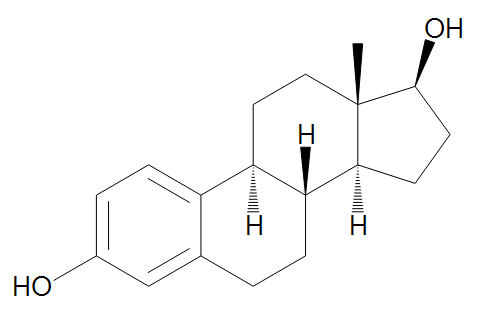
\includegraphics[width=0.48\textwidth]{figuras/estradiol17b.png}
        \label{fig:estradiol}
    }\hfill
    \subfloat[Etinilestradiol]{%
        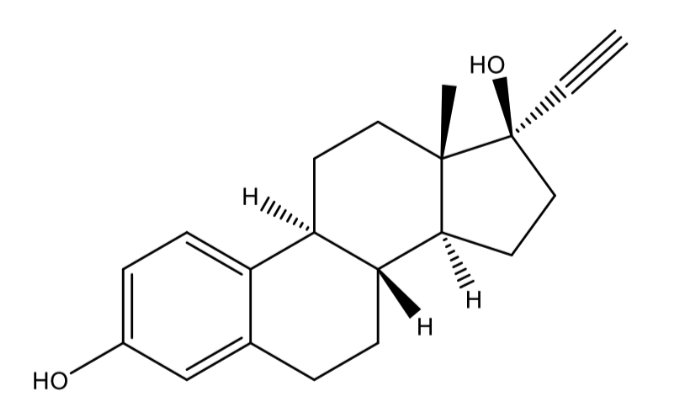
\includegraphics[width=0.48\textwidth]{figuras/etinilestradiol.png}
        \label{fig:etinilestradiol}
        }\par
    \caption[Estradiol 17$\beta$ e etinilestradiol.]{Fórmulas estruturais do estradiol 17$\beta$ \Subfigura{fig:estradiol} e do etinilestradiol \Subfigura{fig:etinilestradiol}.}
    \label{fig:structure}
    \end{center}
\end{figure}

No mercado farmacêutico em todo o mundo, existem diversas fórmulas contendo o etinilestradiol, além de uma variedade de possibilidades de administração, como oral, transdermal e vaginal. A via oral de administração de hormônios contraceptivos é muito bem estabelecida e se trata de comprimidos de administração diária. A via transdermal é realizada através de adesivos aplicados sobre a pele e trocados semanalmente, enquanto a vaginal é feita por um anel de silicone inserido uma vez por mês (Heuvel et al. 2005).

Um grande desafio na indústria farmacêutica diz respeito às matrizes de liberação de medicamentos e sua consistência a longo prazo. Certos fármacos perdem eficácia ao longo do tempo, com sua concentração caindo abaixo do mínimo necessário para a eficácia do tratamento, ou, pelo contrário, acabam ultrapassando a concentração tóxica mínima e produzindo assim efeitos adversos. Por isso, é importante investigar o uso de modelos matemáticos a fim de aprimorar a compreensão da liberação controlada de medicamentos (Simon 2004). A construção desses modelos deve levar em consideração as dinâmicas de absorção do meio, e por isso requer o conhecimento de fenômenos de transporte e transferência de massa (Simon 2007).

\section{Matrizes}

A Organização Mundial da Saúde (OMS) considera o acesso ao planejamento familiar seguro essencial para a promoção da autonomia das mulheres e para a igualdade de gênero. Um elemento citado como fundamental para a qualidade do planejamento familiar é o acesso à escolha entre uma variedade de métodos contraceptivos, bem como à informação para realizar a escolha baseada na eficácia, segurança e benefícios de cada um. Dentre as categorias de escolha recomendadas, estão os \Sigla{contraceptivos hormonais combinados}{CHCs}: as pílulas anticoncepcionais, os adesivos contraceptivos e os anéis vaginais contraceptivos (World Health Organization, 2016).

No mercado mundial, existem diversas fórmulas contendo o etinilestradiol, seja como princípio ativo único ou associado a outro componente, como dienogeste e levonorgestrel, para administração oral (pílula anticoncepcional),  vaginal (anel) ou transdérmica (adesivo). Dependendo da rota de administração, a quantidade de EE na formulação pode variar (Simu et. al., 2022). Sabe-se que os estrogênios possuem efeitos colaterais como dores nos seios, dor de cabeça, retenção de fluidos e náusea, além de trazerem riscos de tromboembolismo (Stanczyk et al., 2013). Contudo, comparando os CHCs, é possível observar entre eles diferenças na exposição ao EE e na ocorrência dos efeitos adversos (Heuvel et al. 2005).

\subsection{Contraceptivos orais combinados}

Os \Sigla{contraceptivos orais combinados}{COCs} têm ajudado milhões de mulheres em todo o mundo a evitar gravidezes não desejadas desde a sua introdução no mercado, nos anos 1960, e seguem hoje sendo a forma de controle de natalidade mais popular. A maior parte dos COCs do passado e presente contém etinilestradiol como componente estrogênico. Para administração oral, o etinilestradiol é usado em uma forma microcristalina a fim de maximizar a superfície de contato, o que possibilita absorção mais eficaz e aumenta sua biodisponibilidade. A formulação do COC pode conter de menos de 20 \textmu g a 30 \textmu g de EE (Kuhl, 2005; Stanczyk et al., 2013). Na \Figura{fig:pills} abaixo, estão dois exemplos de fórmulas comerciais contendo o etinilestradiol em diferentes quantidades.

\begin{figure}[!htb]
    \begin{center}
    \subfloat[Tâmisa\textsuperscript{\textregistered}]{%
        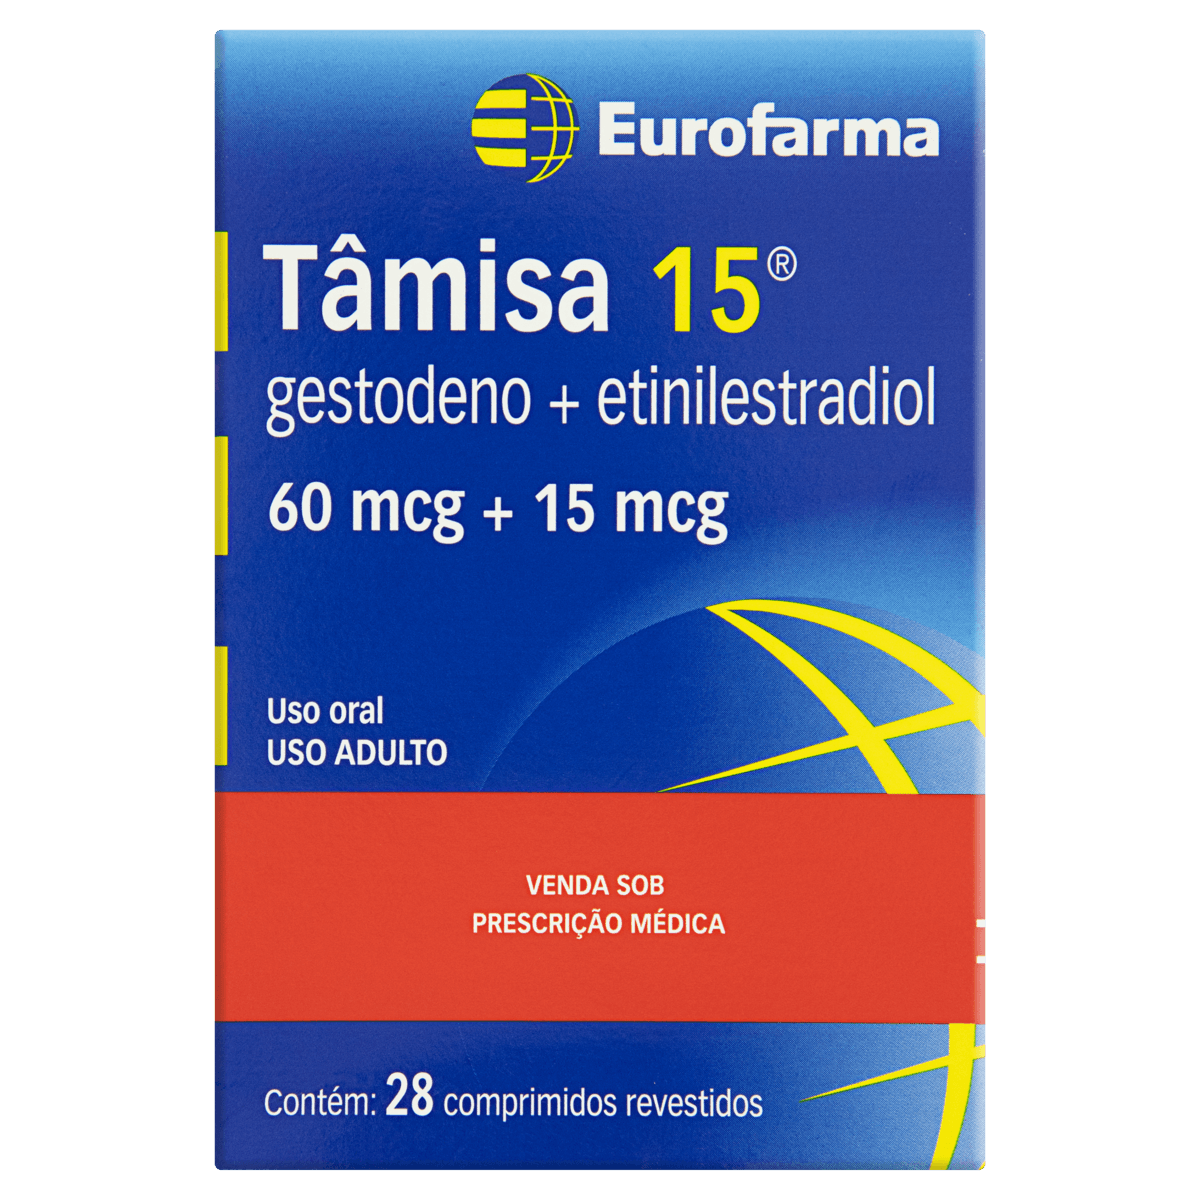
\includegraphics[width=0.28\textwidth]{figuras/Tamisa.png}
        \label{fig:tamisa}
    }\hfill
    \subfloat[Microgynon\textsuperscript{\textregistered}]{%
        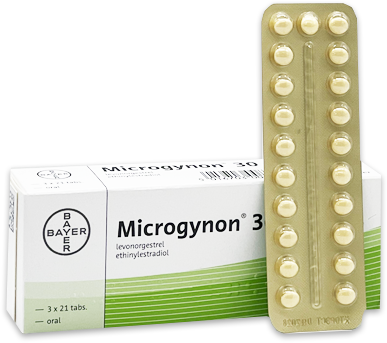
\includegraphics[width=0.28\textwidth]{figuras/Microgynon-Tablets-Side.png}
        \label{fig:microgynon}
        }\par
    \caption[COCs comerciais]{Os COCs Tâmisa\textsuperscript{\textregistered} \Subfigura{fig:tamisa} e Microgynon\textsuperscript{\textregistered}  \Subfigura{fig:microgynon} são exemplos de fórmulas comerciais contendo o etinilestradiol (e-Surgery, 2024; Santa Lúcia Drogarias, 2024).}
    \label{fig:pills}
    \end{center}
\end{figure}

O etinilestradiol é rapidamente absorvido após a administração oral de doses terapêuticas, sendo o pico de concentração plasmática atingido de 1 a 2 horas após a ingestão (Stanczyk et al., 2013). A dosagem diária da pílula produz picos e vales na concentração de EE no sangue ao longo do tempo (Heuvel et al. 2005). A administração oral possui como vantagens o fato de ser fácil e conveniente, não invasiva e rapidamente reversível. Por outro lado, devido à alta atividade metabólica que ocorre no sistema digestivo, são necessárias concentrações mais elevadas do princípio ativo do que em outras matrizes, causando também maior impacto no fígado (Kuhl, 2005).

A maior preocupação existente sobre os COCs diz respeito a seus efeitos colaterais indesejados, principalmente coágulos sanguíneos, ataques cardíacos, AVCs, ganho de peso e perda de libido (Stanczyk et al., 2013). Além disso, sua eficácia depende da ingestão diária correta e consistente, o que acarreta em uma taxa anual de falha de 8\% no uso típico (Lubianca, 2016). 

De acordo com o Ministério da Saúde (s.d.), o Programa Saúde da Mulher disponibiliza comprimidos contendo etinilestradiol para distribuir gratuitamente à população, sendo também parte do Programa Farmácia Popular. Já nas farmácias, o valor de uma caixa de 21 comprimidos pode variar entre R\$18 e R\$96, a depender da composição e do laboratório, segundo dados de Preço Máximo ao Consumidor (PMC) obtidos das Listas de Preços de Medicamentos da ANVISA (2024).

\subsection{Adesivo transdérmico}

O fator do esquecimento e o ônus da ingestão diária de medicamento podem ser contornados pela alternativa da administração de fármacos através da pele, levando o princípio ativo diretamente à circulação sanguínea. Ao evitar a passagem pelo trato gastrointestinal, evita-se também o chamado metabolismo de primeira passagem, fenômeno no qual o fármaco passa pelo fígado antes de entrar na circulação geral, tendo sua concentração reduzida (Scheindlin, 2004; Lin et. al., 2010). Os adesivos transdérmicos foram desenvolvidos com a finalidade de aumentar a adesão e conforto dos pacientes, além de aumentar a biodisponibilidade do fármaco no organismo e possibilitar administração continuada de fármacos com meia-vida curta (Saroha, 2016).

Os adesivos transdérmicos podem ser de dois tipos: matriz ou reservatório. No sistema adesivo em reservatório, o princípio ativo fica em um reservatório líquido, em uma solução de álcool. Já no sistema em matriz, utilizado nos contraceptivos, as moléculas ficam distribuídas uniformemente ao longo de uma matriz polimérica, sendo a difusão do estrogênio para a pele facilitada por alguma substância como um ácido graxo ou etanol. A camada externa é geralmente de poliéster, \Sigla{copolímero etileno acetato de vinila}{EVA} ou poliuretano, enquanto o adesivo é um polímero de acrilato. A taxa de difusão no sistema matricial é mais constante em comparação ao sistema reservatório (Scheindlin, 2004; Kuhl, 2005). A \Figura{fig:patch} mostra uma esquematização das camadas do adesivo do tipo matriz.

\begin{figure}[!htb]
    \centering
        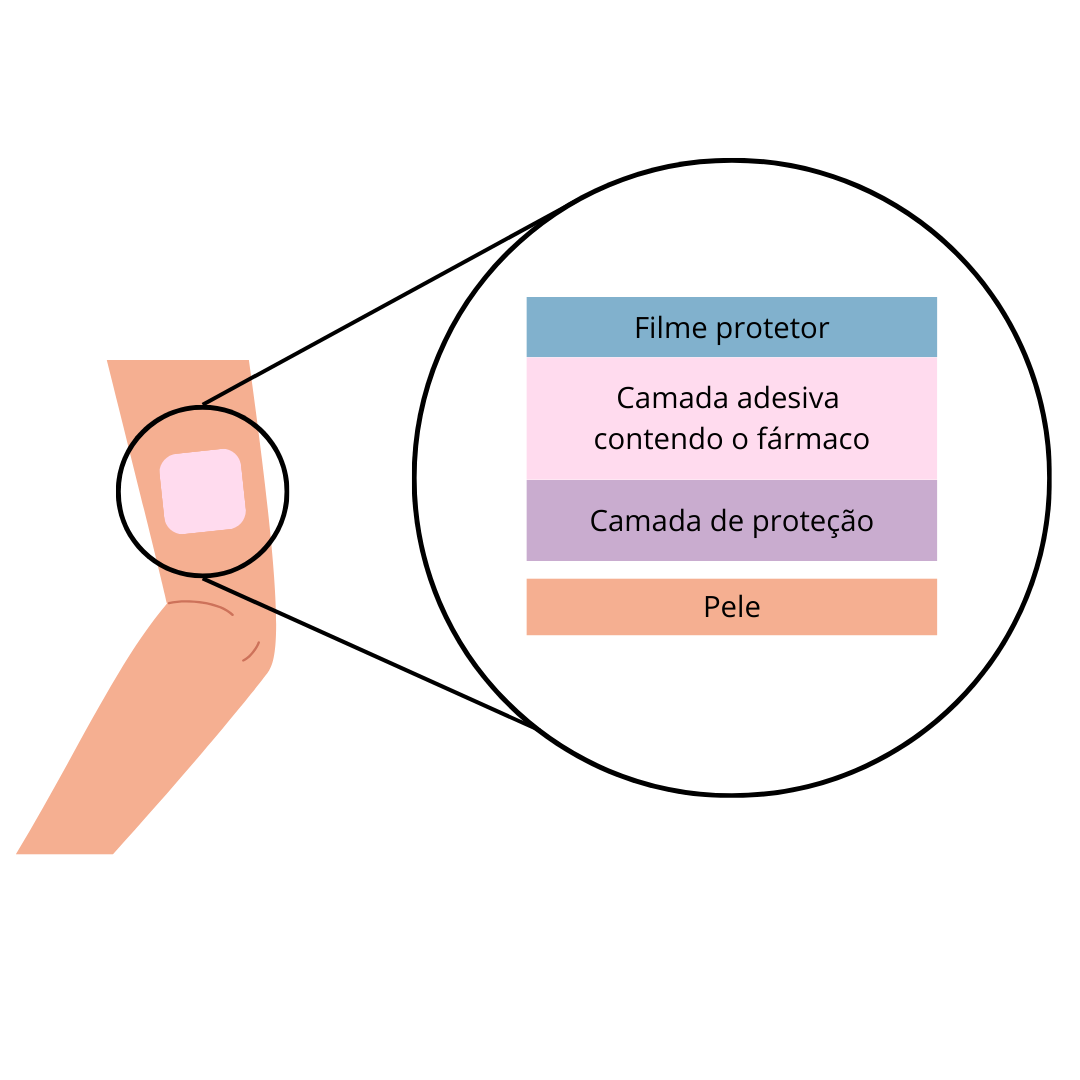
\includegraphics[width=0.48\textwidth]{figuras/adesivo.png}
        \caption[Camadas do adesivo transdérmico do tipo matriz]{Camadas do adesivo transdérmico do tipo matriz. A camada de proteção é removida antes da aplicação (adaptado de Scheindlin, 2004).}
    \label{fig:patch}
\end{figure}

A eficácia da administração de fármacos pela via transdérmica depende da permeabilidade do fármaco em questão na pele. O fluxo é mantido devido a um gradiente de concentração entre o local da aplicação e os capilares sanguíneos. Os pontos negativos da utilização dos adesivos transdérmicos são a dificuldade de ultrapassar a barreira da pele e a possibilidade de reações alérgicas na paciente (Saroha, 2016). Dependendo do tempo que ficam com o adesivo no mesmo local, entre 50 e 60\% das pacientes apresentam vermelhidão de leve a moderada, podendo restar resíduos do adesivo na pele após a retirada (Kuhl, 2005).

Os adesivos contraceptivos são contraceptivos hormonais combinados de aplicação tópica semanal, devendo assim ser aplicados três vezes ao mês. As composições podem variar, podendo chegar a conter 750 \textmu g de etinilestradiol por adesivo (Devineni et. al., 2007). Em geral, os adesivos são projetados para fornecer cerca de 20 \textmu g de EE por dia (Heuvel et al. 2005).

Um estudo de Heuvel et al. (2005) comparando os efeitos da pílula, anel vaginal e adesivo transdérmico contendo etinilestradiol em grupos de mulheres utilizando cada um desses CHCs demonstrou que, apesar de o adesivo ser projetado para fornecer uma dose diária baixa de EE, a exposição ao EE nesse grupo foi a mais alta entre os três, bem como a incidência de efeitos adversos relacionados ao estrogênio. Segundo o estudo, isso pode indicar uma maior eficiência do adesivo em termos de entrega de EE ao corpo, podendo ser utilizado, por exemplo, pelas pacientes que possuem menor sensibilidade aos efeitos colaterais e precisam de uma maior garantia de absorção. 

O adesivo contraceptivo não está incluso entre os medicamentos de distribuição gratuita pelo governo e o preço de uma caixa contendo três adesivos, quantidade suficiente para um mês de contracepção, pode variar entre R\$50 e R\$130 (UOL, 2021; ANVISA, 2024).

\subsection{Anel vaginal}

Os anéis vaginais contraceptivos oferecem, assim como os adesivos transdérmicos, a vantagem de evitar o metabolismo hepático de primeira passagem, oferecendo uso continuado fácil e alta biodisponibilidade de hormônios. Tratam-se de anéis circulares de material polimérico, como o silicone, cuja utilização se dá através da inserção no canal vaginal, onde o dispositivo deve permanecer por 21 dias do mês. O anel vaginal comercial mais conhecido é o NuvaRing{\textregistered}, um anel circular de EVA com estearato de magnésio, que possui 54 mm de diâmetro e 4 mm de espessura, e tem como componente estrogênico o etinilestradiol. Diariamente, o NuvaRing libera para a corrente sanguínea cerca de 15 \textmu g de EE (Barnhart et. al., 2005; Heuvel et al., 2005). A \Figura{fig:nuvaring} mostra o NuvaRing. 

\begin{figure}[!htb]
    \centering
        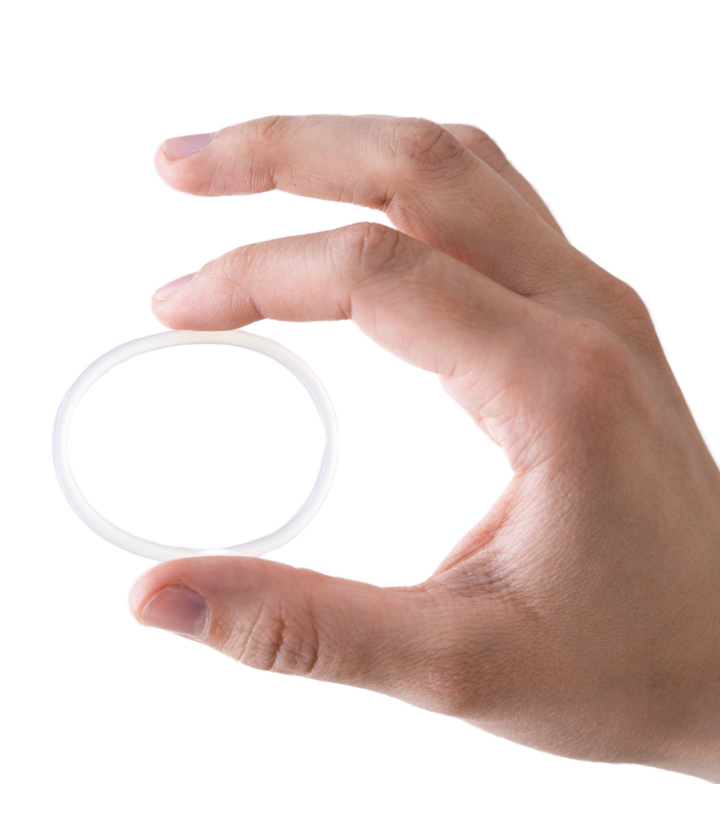
\includegraphics[width=0.38\textwidth]{figuras/nuvaring.png}
        \caption[Anel vaginal]{O anel vaginal contraceptivo NuvaRing{\textregistered} (NuvaRing, 2024).}
    \label{fig:nuvaring}
\end{figure}

O conceito dos anéis vaginais contraceptivos é baseado em dois princípios: a capacidade dos hormônios esteróides, como os estrogênios, de  difundirem lentamente a uma taxa constante através de polímeros biocompatíveis e a capacidade do epitélio do canal vaginal de absorver rapidamente esses hormônios (Faundes et. al, 2004). Por causa disso, a concentração sanguínea de etinilestradiol após a administração vaginal pode ser de 10 a 20 vezes maior do que após a administração oral da mesma dose (Kuhl, 2005).

Dessa forma, a administração pela via vaginal permite uma dosagem baixa, estável e contínua, resultando em uma concentração estável de hormônio no sangue. Isso é benéfico porque minimiza a exposição ao EE, diminuindo a probabilidade da incidência de efeitos colaterais relacionados ao estrogênio (Heuvel et al. 2005). Contudo, a maioria dos dispositivos possui um efeito de liberação inicial rápida antes de atingir um estado estacionário na taxa de liberação, o que provavelmente se deve ao acúmulo de hormônios na superfície do anel durante o armazenamento (Faundes, 2004).

A eficácia contraceptiva do anel vaginal é considerada boa, sendo similar ou um pouco melhor do que a obtida com contraceptivos orais. Ele é fácil de usar, pois necessita de ação por parte da paciente em apenas dois dias por mês, sendo um dia para inserção, no início do ciclo, e outro para retirada, três semanas depois. A conveniência, facilidade e eficácia são as vantagens mais citadas pelas usuárias do anel. Como pontos contrários, estão a inserção no canal vaginal, que pode ser desconfortável ou encontrar resistências culturais em algumas partes do mundo,  além de causar maior probabilidade de sintomas e lesões vaginais em comparação com a utilização dos COCs (Faundes, 2004). 

O estudo comparativo realizado por Heuvel et al. (2005) indicou que o grupo que utilizou o NuvaRing foi o que apresentou a menor variação nos níveis de EE no sangue, em média 3,4 vezes menor do que das pacientes que usaram o adesivo transdérmico e aproximadamente duas vezes menor do que daquelas que usaram o COC. Essas diferenças na farmacocinética do EE entre os diferentes métodos podem ter implicações importantes na escolha do método contraceptivo baseado no perfil de risco e benefício individual de cada paciente.  Os resultados obtidos por esse estudo indicam que a administração vaginal de etinilestradiol com o NuvaRing proporciona uma dosagem muito menor, mais estável e mais precisa do que as vias transdérmica e oral, resultando em uma baixa exposição ao EE e podendo ser indicado a pacientes que possuem sensibilidade aos efeitos do estrogênio. O anel vaginal não está entre os contraceptivos disponíveis gratuitamente pelos programas do governo, e seu valor pode variar entre R\$94 e R\$124 para 1 mês de contracepção (ANVISA, 2024).

\section{Modelagem matemática da liberação de fármacos}

\subsection{Difusão fickiana em membranas orgânicas}

De acordo com a segunda lei da termodinâmica, haverá fluxo de matéria de uma região de maior a outra de menor concentração de uma determinada espécie química, sendo essa espécie denominada soluto. Assim, define-se a transferência de massa como o fenômeno ocasionado pela diferença de concentração, maior para menor, de um determinado soluto em um certo meio. Quando há ação substancial da concentração do soluto no espaço considerado e o transporte ocorre em nível molecular, de forma que a força motriz é o gradiente de concentração, esse fenômeno é conhecido como difusão. Na difusão, a resistência ao transporte está associada somente à interação soluto-meio (Cremasco, 2015).

A difusão pode ocorrer através de membranas, que atuam como barreiras ao transporte, separando dois fluidos e devendo ser vencidas pelo soluto. As membranas podem ser compostas por materiais inorgânicos ou orgânicos, apresentar poros ou não. Na indústria, são utilizadas em diversos processos de separação, tais como adsorção, absorção, secagem, combustão, cristalização, extração, lixiviação e destilação. As membranas feitas de materiais orgânicos são normalmente classificadas como membranas densas, e a descrição da difusão mássica através delas dá-se em virtude das características dos polímeros que as constituem. Esse tipo de membrana é utilizado, por exemplo, na ultrafiltração (Cremasco, 2015; Cremasco, 2019).

As membranas orgânicas, utilizadas normalmente na indústria química e correlatas, são chamadas de membranas isotrópicas densas. Elas são isentas de poros, e o fenômeno da difusão é, portanto, determinado pela interação soluto–polímero. A difusão de um soluto em um polímero ocorre por um processo de estado ativado, via saltos energéticos, ocupando vazios na estrutura polimérica. Tais sítios vagos são fruto do entrelaçamento dos segmentos da cadeia macromolecular, e fazem com que o material se comporte como uma matriz porosa, apesar de não possuir poros fixos. Admitindo que o diâmetro dos poros da estrutura seja muito maior do que o diâmetro de difusão do soluto, e desde que não ocorra variação do volume da matriz, a difusão do soluto em regime permanente será regida pela Primeira Lei de Fick,

\begin{equation}
J_{A,z} = -D_{AB} \frac{dC_A}{dz}
\end{equation}

\noindent sendo $J_{A,z}$ o fluxo de difusão molar do soluto $A$ na direção $z$, $C_A$ a concentração molar do soluto e $D_{AB}$ o coeficiente binário de difusão do soluto A no meio B (Cremasco, 2015; Cremasco, 2019).

\subsection{Difusão na absorção percutânea de fármacos}

A absorção percutânea de fármacos envolve a penetração de um princípio ativo através da pele, sua absorção pelos capilares e distribuição na circulação sistêmica. A Segunda Lei de Fick é comumente utilizada para modelar esse processo. No entanto, diversos fatores importantes precisam ser considerados, como a escolha da membrana, o projeto do sistema de liberação, que simula a aplicação do fármaco, e o tempo de exposição. Além disso, é igualmente essencial contar com uma descrição matemática, que permita prever o comportamento do fármaco com precisão (Simon, 2005).

A Segunda Lei de Fick é representada por uma \Sigla{equação diferencial parcial}{EDP} linear e de segunda ordem que descreve a distribuição de concentração do soluto no tempo e no espaço, para casos em que o regime é transiente e o coeficiente de difusão não depende da concentração do soluto (Cremasco, 2019). Ela é escrita na forma:

\begin{equation}
\frac{\partial C_A}{\partial t} = D_{AB} \frac{\partial^2 C_A}{\partial z^2}
\end{equation}

\noindent e tem sido utilizada na literatura para descrever permeação cutânea de fármacos em que o estado estacionário é atingido após determinado período. Nessa modelagem, tanto a matriz do fármaco quanto a pele são descritas como membranas orgânicas fickianas (Kubota et. al, 2002; Simon, 2005). Kubota et. al (2002) e Simon (2007) utilizaram essa modelagem em seus trabalhos, representando os sistemas como mostrado na \Figura{fig:modelo_adesivo} em que $C_1$ representa a concentração de medicamento na matriz e $C_2$, na pele.

\begin{figure}[!htb]
    \centering
        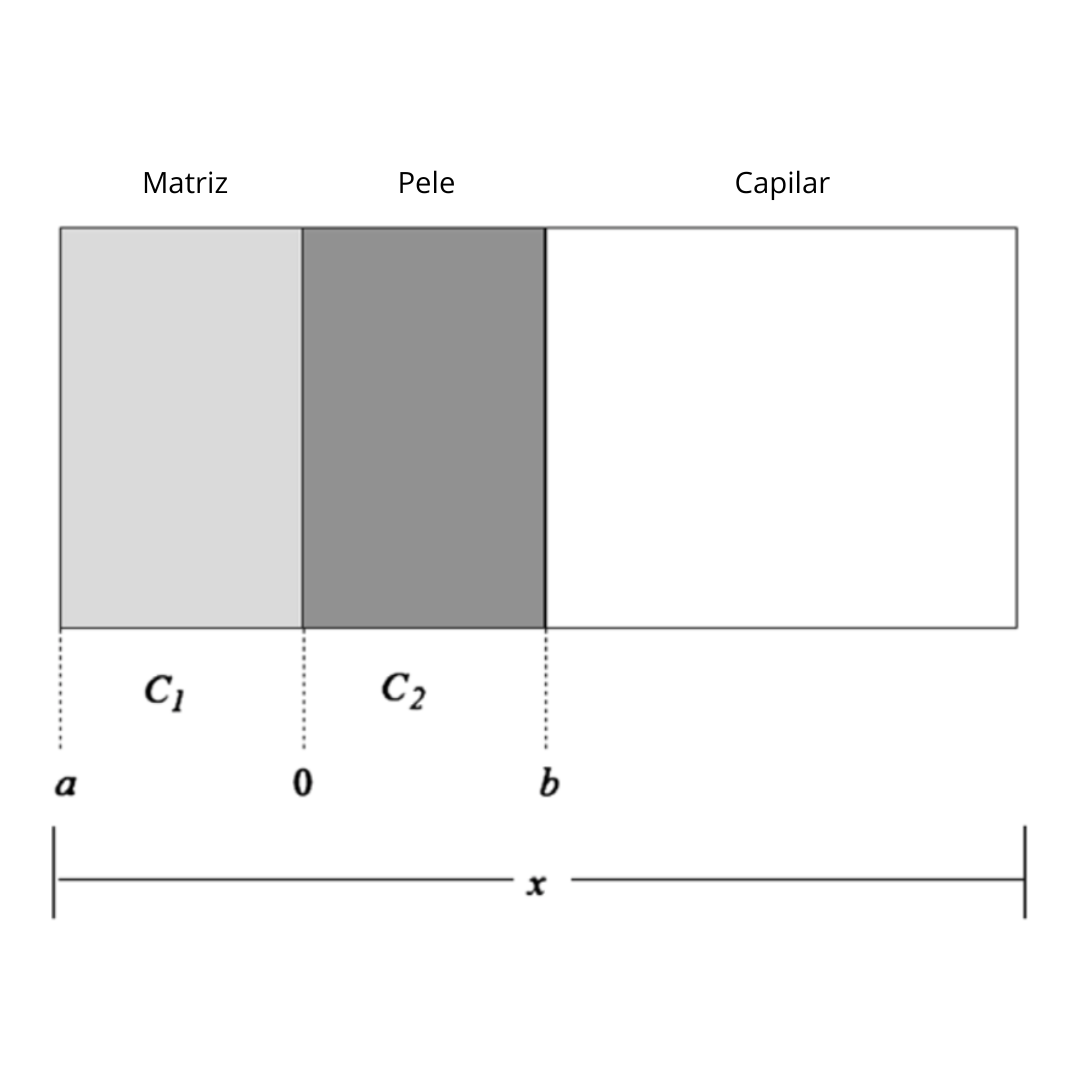
\includegraphics[width=0.48\textwidth]{figuras/modelo_adesivo.png}
        \caption[Representação esquemática de absorção percutânea]{Representação esquemática de absorção percutânea de fármaco (adaptado de Simon, 2007). }
    \label{fig:modelo_adesivo}
\end{figure}

Segundo esse modelo, temos:

\begin{equation}
\frac{\partial C_1}{\partial t} = D_1 \frac{\partial^2 C_1}{\partial x^2}, \quad a < x < 0, \quad 0 < t \leq T
\end{equation}

\begin{equation}
\frac{\partial C_2}{\partial t} = D_2 \frac{\partial^2 C_2}{\partial x^2}, \quad 0 < x < b, \quad 0 < t \leq T
\end{equation}

\noindent em que $D_1$ e $D_2$ são os coeficientes de difusão na matriz e na pele, e $a$ e $b$ são as espessuras da matriz e da pele, respectivamente. $T$ é o período de aplicação.

Simon (2007) ainda definiu as seguintes condições iniciais:

\begin{equation}
C_1[x,0] = C_{10}, \quad a < x < 0
\end{equation}

\begin{equation}
C_2[x,0] = C_{20}, \quad 0 < x < b
\end{equation}

\noindent e as condições de contorno:

\begin{equation}
\frac{\partial C_1(a,t)}{\partial x} = 0, \quad 0 < t \leq T
\end{equation}

\begin{equation}
\frac{D_1\partial C_1[0,t]}{\partial x} = \frac{D_2\partial C_2[0,t]}{\partial x}, \quad 0 < t \leq T
\end{equation}

\begin{equation}
K_m C_1[0,t] = C_2[0,t], \quad 0 < t \leq T
\end{equation}

\begin{equation}
- \frac{D_2\partial C_2[b,t]}{\partial x} = K_{cl}C_2[b,t], \quad 0 < t \leq T
\end{equation}

\noindent em que $K_m$ é o coeficiente de partição matriz-pele e $K_{cl}$ é chamado de \textit{clearance} (depuração) por unidade de área do medicamento por unidade de excesso de concentração em $x = b$. Na Eq. (2.7), garante-se que não ocorre transferência de massa entre a matriz e o ambiente; a Eq. (2.8) representa a continuidade do fluxo através da interface matriz-pele; na Eq. (2.9), tem-se a condição de equilíbrio na interface matriz-pele, e a Eq. (2.10) estabelece que a eliminação do fármaco pelo capilar segue uma cinética de primeira ordem em $x = b$.

O uso de modelos matemáticos auxilia na identificação dos melhores candidatos a componentes de fármacos e dos principais fatores que afetam o transporte dessas substâncias através das barreiras da pele. À medida que os dispositivos transdérmicos se tornam mais sofisticados, cresce a necessidade de inovações tanto na formulação quanto no desenvolvimento de regimes de aplicação eficazes. A fim de acompanhar essa complexidade, são necessários modelos mais elaborados que permitam explicar os fenômenos que ocorrem na administração dos fármacos \textit{in vivo}, contribuindo para otimizar a liberação e a eficácia terapêutica (Simon, 2007).

\subsection{Cinética de primeira ordem}

O modelo da cinética de primeira ordem é utilizado para descrever a absorção e a eliminação de uma variedade de medicamentos. Esse modelo considera que a variação da concentração com o tempo depende apenas  da concentração ($C$) e da constante de liberação de primeira ordem ($K$), segundo a Eq. (2.11) (Bruschi, 2015). 

\begin{equation}
    \frac{dC}{dt} = -KC
\end{equation}

O fenômeno da dissolução de uma partícula sólida em um líquido implica em uma ação superficial, e pode ser descrito pela equação de Noyes-Whitney:

\begin{equation}
    \frac{dC}{dt} = K(C_s - C)
\end{equation}

\noindent onde $C$ é a concentração de soluto no tempo $t$, $C_s$ é a solubilidade no equilíbrio na temperatura do processo, e $K$ é a constante de primeira ordem. Existem diversos sistemas de liberação de fármacos que seguem uma cinética de primeira ordem. Para princípios ativos solúveis incorporados a uma matriz porosa, a quantidade de medicamento liberada é proporcional à quantidade restante na matriz. Dessa forma, a quantidade de princípio ativo liberada tende a diminuir com o tempo (Bruschi, 2015).

%%%%%%%%%%%%%%%%%%%%%%%%%%%%%%%%%%%%%%%%%%%%%%%%%%%%%%%%%%%%%%%%%%

%%%%%%%%%%%%%%%%%%%%%%%%%%%%%%%%%%%%%%%%%%%%%%%%%%%%%%%%%%%%%%%%%%
% O comando a seguir inclui o arquivo desenvolvimento.tex que 
% contém o capítulo de desenvolvimento. 
%%%%%%%%%%%%%%%%%%%%%%%%%%%%%%%%%%%%%%%%%%%%%%%%%%%%%%%%%%%%%%%%%%
\chapter{Metodologia}\label{chp:metodologia}
\section{Modelagem matemática}
\subsection{Adesivo transdérmico}

A modelagem matemática do adesivo transdérmico foi realizada utilizando a Segunda Lei de Fick para descrever a difusão do EE através da camada adesiva, seguindo o modelo de Simon (2007). Dado que o objetivo principal deste trabalho é analisar a difusão do etinilestradiol nas matrizes, e sendo a matriz adesiva a responsável pela liberação controlada do fármaco, tomou-se a decisão de concentrar a análise nessa camada. A difusão do EE através da camada adesiva foi considerada significativamente mais lenta do que a absorção na pele e nos vasos sanguíneos, representando a etapa limitante do processo. Dessa forma, optou-se por desconsiderar a camada da pele, simplificando o modelo sem perda de representatividade para o caso limite do estudo. Assim, foi considerada apenas a EDP correspondente à camada adesiva:

\begin{equation}
\frac{\partial C_1}{\partial t} = D_1 \frac{\partial^2 C_1}{\partial x^2}, \quad 0 < x < L_1, \quad 0 < t \leq T
\end{equation}

\noindent sendo $C_1$ a concentração de etinilestradiol e $D_1$ o coeficiente de difusão na camada adesiva, $L_1$ a espessura da camada e $T$ o período de aplicação.

A fim de calcular a concentração inicial, foi primeiro calculado o volume ocupado pela camada adesiva. Para isso, foi utilizado o valor de 0,004 cm para a espessura do adesivo (Simon, 2007) e a área superficial de 20 cm\textsuperscript{2} (Devineni, 2007).

\begin{equation}
    V = A \cdot L_1 
\end{equation}
\begin{equation}
    V = 20 \cdot 0,004 = 0,08 cm\textsuperscript{3}
\end{equation}

A dosagem considerada foi de 750 \textmu g de etinilestradiol por adesivo (Devineni, 2007) e supõe-se que a concentração seja uniforme ao longo da matriz. Dessa forma, a concentração inicial pode ser obtida por: 

\begin{equation}
C_1[x,0] = C_{10}, \quad 0 < x < L_1
\end{equation}
\begin{equation}
    C_{10} = \frac{750 \, \mu g}{0,08 \, cm\textsuperscript{3}} =  9375 \, \mu g/cm\textsuperscript{3}
\end{equation}

Para o coeficiente de difusão, foi considerado o trabalho de Rohr e Saeger‐Lorenz (2002), no qual foi estudado o coeficiente de difusão do $17\beta$-estradiol em uma matriz adesiva. Devido à ausência de dados na literatura sobre o coeficiente de difusão do etinilestradiol nesse tipo de matriz, foi necessário realizar uma aproximação a partir desse valor. Sabe-se que o coeficiente de difusão é influenciado por vários fatores, entre eles o tamanho, a forma e a flexibilidade da molécula em difusão. Sabe-se também que seu valor é inversamente proporcional ao raio da molécula (Kreilgaard et. al, 2000). Assim, devido à adição do grupo etinil causar aumento do raio da molécula, considera-se esse valor como uma aproximação inicial, sendo que o coeficiente de difusão real do etinilestradiol será um valor menor a ser determinado empiricamente durante a modelagem computacional. Convertendo o valor obtido na literatura para cm\textsuperscript{2}/h, tem-se:

\begin{equation}
    D_1 = 7,2 \times 10^{-11} \, cm\textsuperscript{2}/s \times 3600 \, \text{s/h} = 2,59 \times 10^{-7} \, cm\textsuperscript{2}/h
\end{equation}

Para as condições de contorno, foi considerado que na borda exterior, $x = 0$, o fluxo é nulo, devido ao sistema possuir uma quantidade finita de fármaco. Na borda mais próxima da pele, $x = L$, foi definida uma condição de partição utilizando coeficiente $Km = 1$ (Simon, 2007), indicando que a concentração do fármaco é a mesma na matriz e na pele em equilíbrio. Essas condições podem ser visualizadas na Eq. (3.7) e Eq. (3.8) abaixo.

\begin{equation}
\frac{\partial C_1(0,t)}{\partial x} = 0, \quad 0 < t \leq T
\end{equation}

\begin{equation}
K_m C_1(L_1,t) = C_{pele}, \quad 0 < t \leq T
\end{equation}

A \Tabela{tab:tabela_1} contém um resumo dos parâmetros utilizados nesse modelo.

\begin{table}[!htp]
\caption[Parâmetros para o adesivo transdérmico]{Parâmetros utilizados para o modelo do adesivo transdérmico}
\label{tab:tabela_1}
\begin{center}
\begin{tabular}{ccc}
\toprule % Linha superior
Parâmetro & Valor & Referência \\ \midrule % Linha do meio 
\textbf{$D_1$}  & $5,184 \times 10^{-8} \, cm\textsuperscript{2}/h$ & Rohr e Saeger-Lorenz (2002) \\
\textbf{$C_{10}$} & 9375 \textmu g/cm\textsuperscript{3} & Devineni (2007) \\
\textbf{$L_1$}  & 0,004 cm & Simon (2007) \\
\textbf{$K_m$} & 1 & Simon (2007) \\\bottomrule % Linha inferior
\end{tabular}
\end{center}
\end{table}

\subsection{Anel vaginal}

A modelagem matemática do anel vaginal foi realizada de maneira análoga à da camada adesiva, sendo sua EDP correspondente:

\begin{equation}
\frac{\partial C_2}{\partial t} = D_2 \frac{\partial^2 C_2}{\partial x^2}, \quad 0 < x < L_2, \quad 0 < t \leq T
\end{equation}

A fim de calcular a concentração inicial, foi necessário primeiro calcular o volume do anel. O anel vaginal pode ser definido como um toróide oco, conforme mostra a \Figura{fig:anel_vaginal} abaixo:

\begin{figure}[!htb]
    \centering
        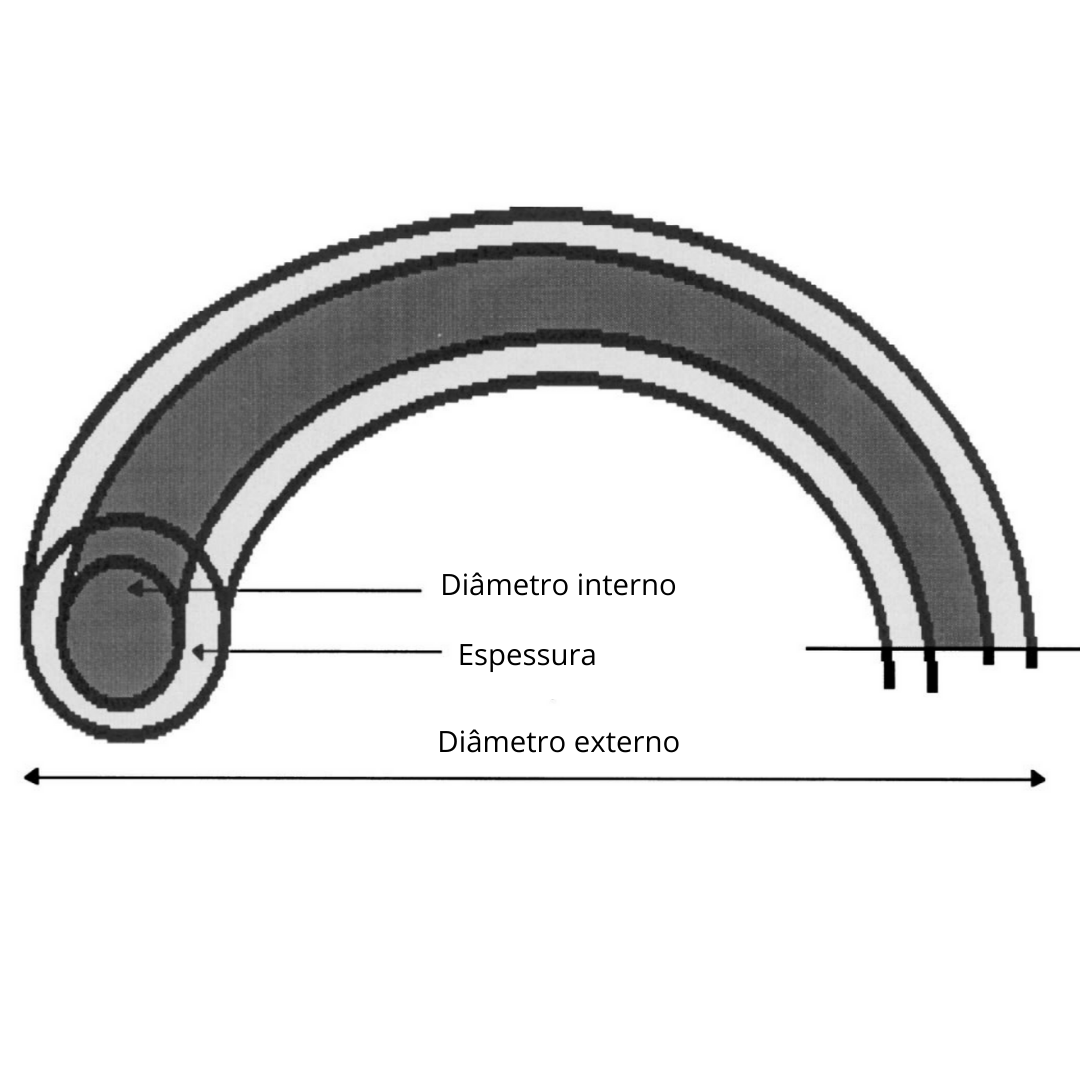
\includegraphics[width=0.48\textwidth]{figuras/anel_vaginal.png}
        \caption[Geometria de um anel vaginal]{Geometria de um anel vaginal (Woolfson et. al, 1999).}
    \label{fig:anel_vaginal}
\end{figure}

Assim, é necessário calcular o volume do toróide externo e subtrair o volume do toróide interno. De Barnhart et. al (2005), de acordo com as especificações do NuvaRing{\textregistered}, temos que $D_{ext} = 54 \, mm$ e $e = 4 \, mm$. Calculando os raios externo ($R_{ext}$) e interno ($R_{int}$), em centímetros:

\begin{equation}
R_{ext} = \frac{D_{ext}}{2} = \frac{54}{2 \cdot 10} = 2,7 \, cm
\end{equation}

\begin{equation}
R_{int} = R_{ext} - e = 2,7 - \frac{4}{10} = 2,3 \, cm
\end{equation}

Subtraindo a área da seção interna da área da seção externa, e multiplicando pelo comprimento da circunferência:

\begin{equation}
V = \pi \cdot (R_{ext}^2 - R_{int}^2) \cdot 2 \cdot \pi \cdot R_{ext} = 106,58 \, cm\textsuperscript{3}
\end{equation}

A quantidade de etinilestradiol presente em um anel é de 2,7 mg (Banhart et. al, 2005), e supõe-se uma concentração uniforme ao longo de seu volume. Dessa forma, a concentração inicial pode ser obtida por: 

\begin{equation}
C_2[x,0] = C_{20}, \quad 0 < x < L_2
\end{equation}
\begin{equation}
    C_{20} = \frac{2700 \, \mu g}{106,58 \, cm\textsuperscript{3}} =  25,33 \, \mu g/cm\textsuperscript{3}
\end{equation}

O coeficiente de difusão $D_2$ foi obtido de Malcom et. al (2003). O valor é referente à difusão do $17\beta$-estradiol em um anel vaginal feito de silicone, material diferente do NuvaRing, que é de EVA. Novamente, devido à ausência de dados específicos para o etinilestradiol em um anel de EVA, faz-se a consideração de que esse valor é uma aproximação inicial razoável devido à similaridade dos compostos envolvidos, a ser reavaliada posteriormente. Convertendo o valor obtido na literatura para cm\textsuperscript{2}/h, tem-se:

\begin{equation}
D_2 = 1,1 \times 10^{-6} \, cm\textsuperscript{2}/s \times 3600 \, \text{s/h} = 3,96 \times 10^{-3} \, cm\textsuperscript{2}/h
\end{equation}

Para o anel vaginal, também foi adotada uma condição de contorno de fluxo zero na borda exterior, $x = 0$, e, na borda $x = L$, a concentração foi definida como zero, a fim de simular o fluxo livre do fármaco na interface matriz-pele, dada a absorção rápida que ocorre na região (Faundes, 2004). Essas condições podem ser visualizadas na Eq. (3.16) e Eq. (3.17) abaixo.

\begin{equation}
\frac{\partial C_2(0,t)}{\partial x} = 0, \quad 0 < t \leq T
\end{equation}

\begin{equation}
C_2(L_2,t) = 0, \quad 0 < t \leq T
\end{equation}

A \Tabela{tab:tabela_2} contém um resumo dos parâmetros utilizados no modelo do anel vaginal.

\begin{table}[!htp]
\caption[Parâmetros para o anel vaginal]{Parâmetros utilizados para o modelo do anel vaginal}
\label{tab:tabela_2}
\begin{center}
\begin{tabular}{ccc}
\toprule % Linha superior
Parâmetro & Valor & Referência \\ \midrule % Linha do meio 
\textbf{$D_2$}  & $3,96 \times 10^{-3} \, cm\textsuperscript{2}/h$ & Malcom et. al (2003) \\
\textbf{$C_{20}$} & $25,33 \, \mu g/cm\textsuperscript{3}$ & Barnhart et. al (2005) \\
\textbf{$L_2$}  & 0,4 cm & Barnhart et. al (2005) \\\bottomrule % Linha inferior
\end{tabular}
\end{center}
\end{table}

\subsection{Contraceptivo oral combinado}

A modelagem matemática para a liberação do etinilestradiol a partir do COC, ou pílula anticoncepcional, foi realizada utilizando a equação de Noyes-Whitney para descrever a cinética de dissolução de primeira ordem do EE no fluido gastrointestinal, segundo a Eq. (3.18):

\begin{equation}
    \frac{dC_3}{dt} = k_d (C_s - C_3)
\end{equation}

\noindent sendo $C_3$ a concentração do EE no fluido gastrointestinal, $C_s$ sua solubilidade nesse fluido e $k_d$ a constante de dissolução.

Foi estabelecida a condição inicial de uma concentração nula de EE no fluido gastrointestinal, portanto:

\begin{equation}
    C_3(0) = 0
\end{equation}

O parâmetro $C_s$ foi obtido do artigo de Teleki et al. (2020), que relatou uma solubilidade de 18,7 \textmu g/mL para o EE em uma solução preparada com o objetivo de simular as condições do fluido gastrointestinal. 

Já para a constante de dissolução ($k_d$), foi utilizada uma aproximação a partir da constante de absorção ($k_a$), calculado através dos parâmetros cinéticos $t_{max}$ e $t_{\frac{1}{2}}$, que correspondem, respectivamente, ao tempo para atingir a concentração máxima e ao tempo de meia-vida. De Currie (2018), temos as relações farmacocinéticas:

\begin{equation}
    k_a = \frac{\ln(k_e) + t_{\text{max}} \cdot k_e}{t_{\text{max}}}
\end{equation}

\begin{equation}
    k_e = \frac{\ln(2)}{t_{\frac{1}{2}}}
\end{equation}

Em Heuvel et al. (2005), foram encontrados valores para $t_{max}$ e $t_{\frac{1}{2}}$ do etinilestradiol em um COC. Substituindo $t_{\frac{1}{2}}$ na Eq. (3.21):

\begin{equation}
    k_e = \frac{\ln(2)}{24,4} = 0,0284 \, \text{h}^{-1}
\end{equation}

Substituindo esse resultado na Eq. (3.20), bem como o valor de $t_{max}$, é possível calcular a constante de absorção $k_a$:

\begin{equation}
    k_a = \frac{\ln(0,0284) + 386 \cdot 0,0284}{386} = 0,019 \, \text{h}^{-1}
\end{equation}

Finalmente, é realizada uma aproximação de $k_d$ a partir de $k_a$, a partir da consideração de que todo o EE dissolvido será absorvido:

\begin{equation}
    k_d \approx k_a = 0,019 \, \text{h}^{-1}
\end{equation}

A \Tabela{tab:tabela_3} contém um resumo dos parâmetros utilizados nesse modelo.

\begin{table}[!htp]
\caption[Parâmetros para o COC]{Parâmetros utilizados para o modelo do comprimido oral combinado}
\label{tab:tabela_3}
\begin{center}
\begin{tabular}{ccc}
\toprule % Linha superior
Parâmetro & Valor & Referência \\ \midrule % Linha do meio 
\textbf{$C_s$}  & 18,7 \textmu g/cm\textsuperscript{3} & Teleki et al. (2020) \\
\textbf{$t_{max}$} & 386 h & Heuvel et al. (2005) \\
\textbf{$t_{\frac{1}{2}}$} & 24,4 h & Heuvel et al. (2005) \\\bottomrule % Linha inferior
\end{tabular}
\end{center}
\end{table}

\section{Modelagem computacional}

\subsection{Adesivo transdérmico e anel vaginal}

A modelagem computacional para a difusão no adesivo transdérmico e no anel vaginal foi realizada a partir de uma abordagem similar, devido a ambos os sistemas serem descritos por equações diferenciais parciais. Para cada um, foram utilizados os parâmetros descritos na seção anterior. O tempo total da simulação utilizado para cada matriz foi o tempo de permanência no corpo, ou seja, 168 horas (1 semana) para o adesivo e 504 horas (3 semanas) para o anel.

\phantomsection

\subsubsection{Método das diferenças finitas}

Inicialmente, foi aplicado o método das diferenças finitas, conforme descrito em Lona (2018). Esse método consiste em transformar a EDP em uma equação mais fácil de resolver através de discretizações no tempo e espaço.

Considerando a EDP utilizada para a concentração nas matrizes

\begin{equation}
    \frac{\partial C}{\partial t} = D \frac{\partial^2 C}{\partial x^2}
\end{equation}

Dado que a o valor inicial da concentração é conhecido nos dois casos, pode-se representar o valor em qualquer ponto em função de um incremento infinitesimal em $i$ no caso do espaço e em $j$ no caso do tempo, de acordo com a visualização na \Figura{fig:grid}.

\begin{figure}[!htb]
    \centering
        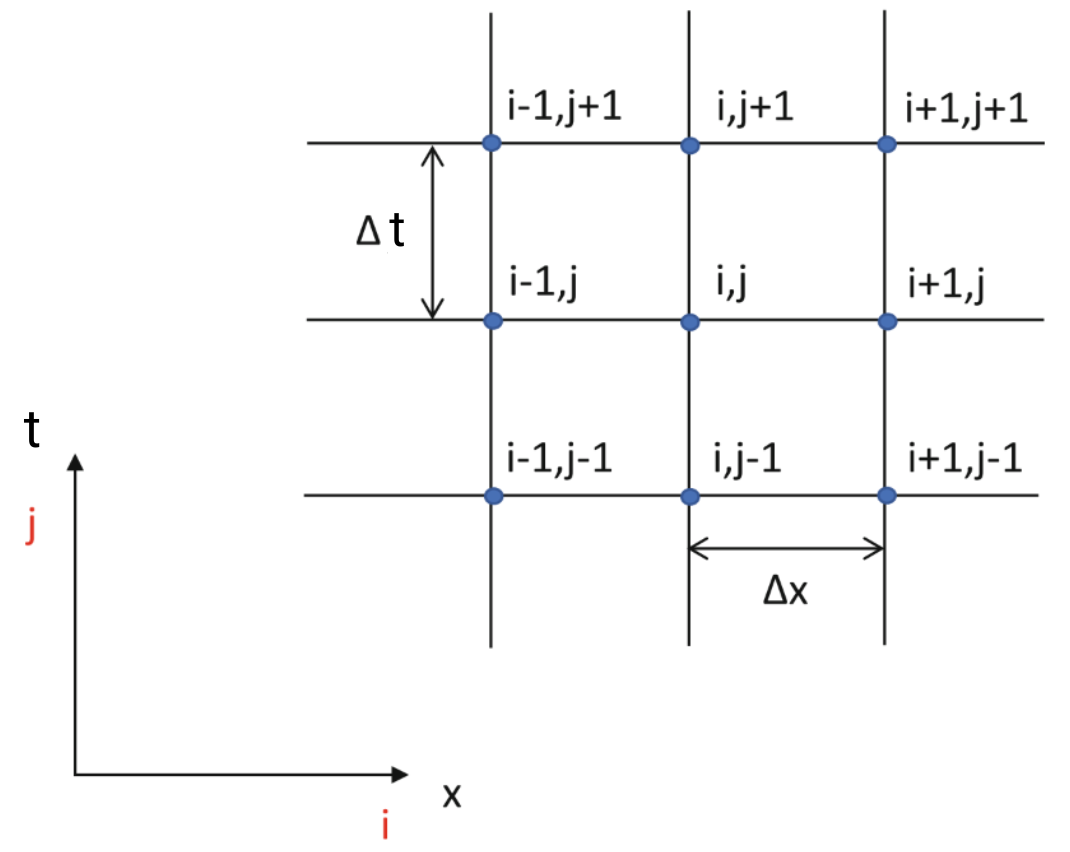
\includegraphics[width=0.48\textwidth]{figuras/grid.png}
        \caption[Grade para visualização do método das diferenças finitas]{Grade para visualização do método das diferenças finitas (adaptado de Lona, 2018).}
    \label{fig:grid}
\end{figure}

Portanto, discretizando as derivadas parciais, temos:

\begin{equation}
    \left( \frac{\partial C}{\partial t} \right)_{i,j} = \frac{C_{i,j+1} - C_{i,j}}{\Delta t}
\end{equation}

\begin{equation}
    \left( \frac{\partial^2 C}{\partial x^2} \right)_{i,j} = \frac{C_{i-1,j} - 2C_{i,j} + C_{i+1,j}}{(\Delta x)^2}
\end{equation}

Substituindo na equação original:

\begin{equation}
    \frac{C_{i,j+1} - C_{i,j}}{\Delta t} = D \frac{C_{i+1,j} - 2C_{i,j} + C_{i-1,j}}{(\Delta x)^2}
\end{equation}

Rearranjando para resolver $C_i^{j+1}$:

\begin{equation}
    C_i^{j+1} = C_i^j + \frac{D \Delta t}{\Delta x^2} (C_{i+1}^j - 2C_i^j + C_{i-1}^j)
\end{equation}

O método de diferenças finitas é amplamente utilizado para problemas de difusão e demais situações de estado transiente, devido à facilidade de implementação. Porém, trata-se de um método condicionalmente estável, ou seja, sua estabilidade está sujeita à chamada condição de \Sigla{Courant–Friedrich–Lecy}{CFL}, dada por:

\begin{equation}
    k \frac{\Delta t}{\Delta x^2} \leq \frac{1}{2}
\end{equation}

\noindent onde $k$ é um parâmetro característico do problema, que aqui corresponde ao coeficiente de difusão (Chicone, 2017). Nessa condição, o passo temporal ($\Delta t$) depende do menor comprimento da célula no domínio computacional, tornando-a muito restritiva para resolver problemas com materiais finos (Chung et. al, 2003). 

Devido à espessura das matrizes poliméricas tanto do adesivo transdérmico quanto do anel vaginal serem muito pequenas, foi necessário um número extremamente alto de pontos temporais para satisfazer a condição CFL. Isso, somado aos altos valores de tempo total da simulação, resultou em consumo excessivo de memória e longos tempos de execução, tornando inviável a utilização do método das diferenças finitas.

\subsubsection{Método de Crank-Nicolson}

Crank (1975) propõe o uso do método de Crank-Nicolson como alternativa para o método das diferenças finitas em problemas de difusão. Enquanto o método de diferenças finitas padrão utiliza o estado da variável em um instante de tempo específico, o método de Crank-Nicolson faz uma média entre o instante atual e o próximo, combinando informações dos estados em $j$ e $j+1$, aplicando diferenças finitas tanto no tempo quanto no espaço. A aproximação da derivada espacial passa a ser dada por:

\begin{equation}
\frac{C_i^{j+1} - C_i^j}{\Delta t} = D \frac{C_{i+1}^{j+1} - 2C_i^{j+1} + C_{i-1}^{j+1} + C_{i+1}^j - 2C_i^j + C_{i-1}^j}{2 \Delta x^2}
\end{equation}

\noindent onde:
\begin{itemize}
    \item \( C_i^j \) representa a concentração no ponto \( i \) e no instante \( j \),
    \item \( \Delta t \) é o intervalo de tempo,
    \item \( \Delta x \) é o passo espacial.
\end{itemize}

A equação acima pode ser reorganizada para obter a forma explícita da concentração em $j+1$:

\begin{equation}
- \frac{\alpha}{2} C_{i-1}^{j+1} + (1 + \alpha) C_i^{j+1} - \frac{\alpha}{2} C_{i+1}^{j+1} = \frac{\alpha}{2} C_{i-1}^j + (1 - \alpha) C_i^j + \frac{\alpha}{2} C_{i+1}^j
\end{equation}

\noindent onde \( \alpha = \frac{D \Delta t}{\Delta x^2} \).

Esta equação resulta em um sistema tridiagonal que pode ser resolvido para cada instante \( j+1 \). Em termos matriciais, pode-se representar o sistema linear para os valores de \( C_i^{j+1} \) da seguinte forma:

\[
\begin{pmatrix}
1 + \alpha & -\frac{\alpha}{2} & 0 & \cdots & 0 \\
-\frac{\alpha}{2} & 1 + \alpha & -\frac{\alpha}{2} & \cdots & 0 \\
0 & -\frac{\alpha}{2} & 1 + \alpha & \cdots & 0 \\
\vdots & \vdots & \vdots & \ddots & \vdots \\
0 & 0 & 0 & -\frac{\alpha}{2} & 1 + \alpha \\
\end{pmatrix}
\begin{pmatrix}
C_1^{j+1} \\
C_2^{j+1} \\
C_3^{j+1} \\
\vdots \\
C_n^{j+1}
\end{pmatrix}
=
\begin{pmatrix}
b_1 \\
b_2 \\
b_3 \\
\vdots \\
b_n
\end{pmatrix}
\]

\noindent onde, para cada ponto:

\[
b_i = \frac{\alpha}{2} C_{i-1}^j + (1 - \alpha) C_i^j + \frac{\alpha}{2} C_{i+1}^j.
\]

Esse tipo de método, em que as soluções de um conjunto de equações simultâneas são obtidas para cada passo temporal, é chamado método implícito. Apesar de envolver mais trabalho para calcular cada ponto, o método de Crank-Nicolson garante estabilidade para todo valor de $\alpha$, sem precisar satisfazer a condição CFL. Isso permite usar passos temporais maiores, conforme necessário (Crank, 1975). Assim, foi possível obter uma modelagem melhor para o adesivo e o anel, exigindo menos recursos computacionais e otimizando o tempo de execução. 

Finalmente, foram adicionadas verificações para garantir que a quantidade de EE liberada em um único dia não ultrapassasse os valores da literatura, sendo 20 \textmu para o adesivo e  15 \textmu para o anel (Barnhart et. al., 2005; Heuvel et al. 2005), e que a quantidade total liberada não ultrapassasse a quantidade de fármaco disponível na matriz. Dessa forma, o modelo se aproxima mais das restrições físicas conhecidas.

Os modelos foram implementados em Python, utilizando o ambiente do Google Colab. Foram plotados gráficos para a concentração ao longo de cada uma das matrizes, em diferentes períodos de tempo. Os códigos completos para esses modelos encontram-se no Apêndice A, nas seções A.1 e A.2.

\subsection{Contraceptivo oral combinado}

A liberação de etinilestradiol a partir da pílula anticoncepcional (COC) é representada pela \Sigla{equação diferencial ordinária}{EDO}:

\begin{equation}
    \frac{dC}{dt} = k_d (C_s - C)
\end{equation}

\noindent sendo que a concentração inicial é conhecida ($C = 0$). 

Para resolvê-la, optou-se por um método numérico que simula a expansão da EDO em série de Taylor, utilizada na solução analítica, sem a necessidade de calcular derivadas de ordem superior. Trata-se do método de Runge-Kutta de quarta ordem (RK4), que é altamente preciso, computacionalmente eficiente e de implementação relativamente simples. A expressão geral para esse método foi obtida a partir de Lona (2018), e está descrita a seguir.

\begin{equation}
    y_{i+1} = y_i + \frac{h}{6} (K_1 + 2K_2 + 2K_3 + K_4) 
\end{equation}

\noindent onde $h$ é o passo temporal e $K_1$, $K_2$, $K_3$ e $K_4$ são as primeiras quatro derivadas:

\begin{equation}
\begin{aligned}
    K_1 &= f(x_i, y_i) \\
    K_2 &= f(x_i + 0.5h, \, y_i + 0.5h K_1) \\
    K_3 &= f(x_i + 0.5h, \, y_i + 0.5h K_2) \\
    K_4 &= f(x_i + h, \, y_i + h K_3)
\end{aligned}
\end{equation}

Para refinar os resultados de acordo com a realidade física, foi adicionada uma restrição para que a concentração liberada não ultrapassasse a quantidade de princípio ativo disponível em uma pílula. 

O modelo também foi implementado em Python, com o objetivo de obter um gráfico da concentração de etinilestradiol no fluido gastrointestinal ao longo do tempo. O código encontra-se no Apêndice A, na seção A.3.

\subsection{Taxa de liberação}

Durante o desenvolvimento do modelo, definiu-se como foco o estudo da liberação do etinilestradiol a partir de cada uma das matrizes. Portanto, a fim de calcular a concentração liberada ao longo do tempo, não foram considerados quaisquer processos metabólicos que pudessem influenciar nesse valor, como a distribuição, a eliminação e a absorção do fármaco no corpo humano.

 A taxa de liberação é calculada tomando a diferença entre as concentrações em intervalos consecutivos de tempo. Para o adesivo transdérmico e o anel vaginal, foi utilizada, para cada ponto temporal, a média da concentração ao longo de todos os pontos espaciais naquele instante. Com isso, para todos os modelos, foi seguida a expressão:

\begin{equation}
    R(t) = \Delta C = C_t - C_{t-1}
\end{equation}

\noindent onde $R$ é a taxa de liberação em um instante $t$.

Foram plotados os gráficos de liberação para cada matriz separadamente utilizando o intervalo de aplicação de cada uma. Em seguida, foi plotado um único gráfico para todas, utilizando o maior intervalo de tempo (21 dias) e considerando reposições para a pílula e o adesivo. O código completo encontra-se na seção A.4 do Apêndice A.
\chapter{Resultados e discussão}\label{chp:resultados}

\section{Difusão de etinilestradiol nas matrizes poliméricas}

A \Figura{fig:difusao_adesivo} mostra a difusão de EE ao longo da camada polimérica do anel vaginal (posição em \textmu m) em diferentes dias, para $D_1 = 5,76 \times 10^{-13}$.  A concentração de EE permanece alta na maior parte da matriz, com uma diminuição acentuada nas bordas, refletindo as condições de contorno impostas e indicando uma maior resistência para a difusão.

Já na \Figura{fig:difusao_anel}, pode ser observada a difusão de EE ao longo da camada polimérica (posição em cm) em cada semana, para $D_2 = 7,92 \times 10^{-7}$. Nesse caso, a concentração de EE diminui gradualmente ao longo das semanas, indicando uma liberação contínua do fármaco.

\begin{figure}[!htb]
    \centering
        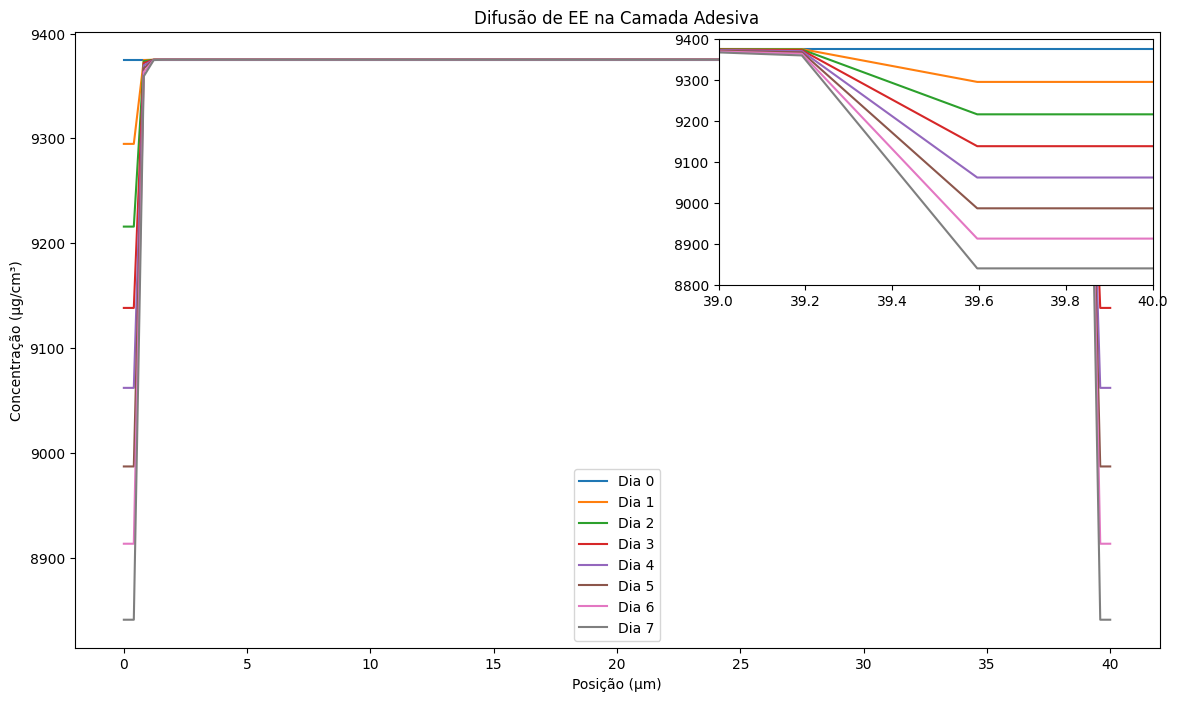
\includegraphics[width=1\textwidth]{figuras/difusao_adesivo.png}
        \caption[Difusão de etinilestradiol ao longo da camada adesiva]{Perfil obtido para a difusão de etinilestradiol ao longo da camada adesiva, para $D_1 = 5,76 \times 10^{-13}$. No canto superior direito, tem-se a região da extremidade ($0 < x < 1\mu m$) ampliada para melhor visualização da variação de concentração ao longo dos dias.}
    \label{fig:difusao_adesivo}
\end{figure}

\begin{figure}[!htb]
    \centering
        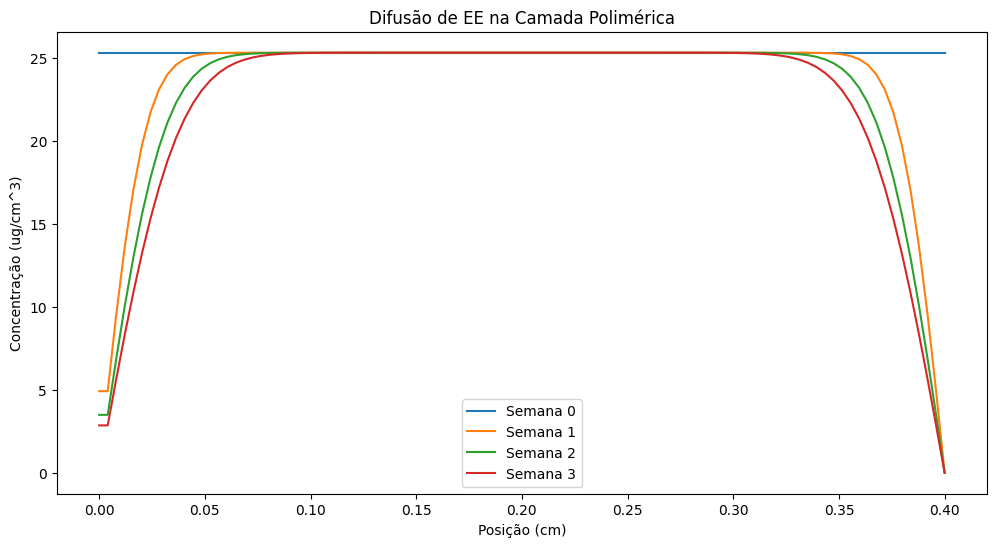
\includegraphics[width=1\textwidth]{figuras/difusao_anel.png}
        \caption[Difusão de etinilestradiol ao longo da camada polimérica do anel]{Perfil obtido para a difusão de etinilestradiol ao longo da camada polimérica do anel vaginal, para $D_2 = 7,92 \times 10^{-7}$.}
    \label{fig:difusao_anel}
\end{figure}

Ambos os perfis podem ser comparados com a \Figura{fig:Higuchi1961}, de Higuchi (1961), que esquematiza a difusão de um soluto de uma matriz polimérica para um fluido assumido como um sumidouro perfeito, fazendo com que a concentração de soluto nunca se acumule o suficiente para alterar a força motriz da difusão. Essa condição é válida para situações em que a concentração do soluto é muito maior do que a concentração de saturação, ou seja, a matriz está inicialmente saturada com soluto dissolvido. 

\begin{figure}[!htb]
    \centering
        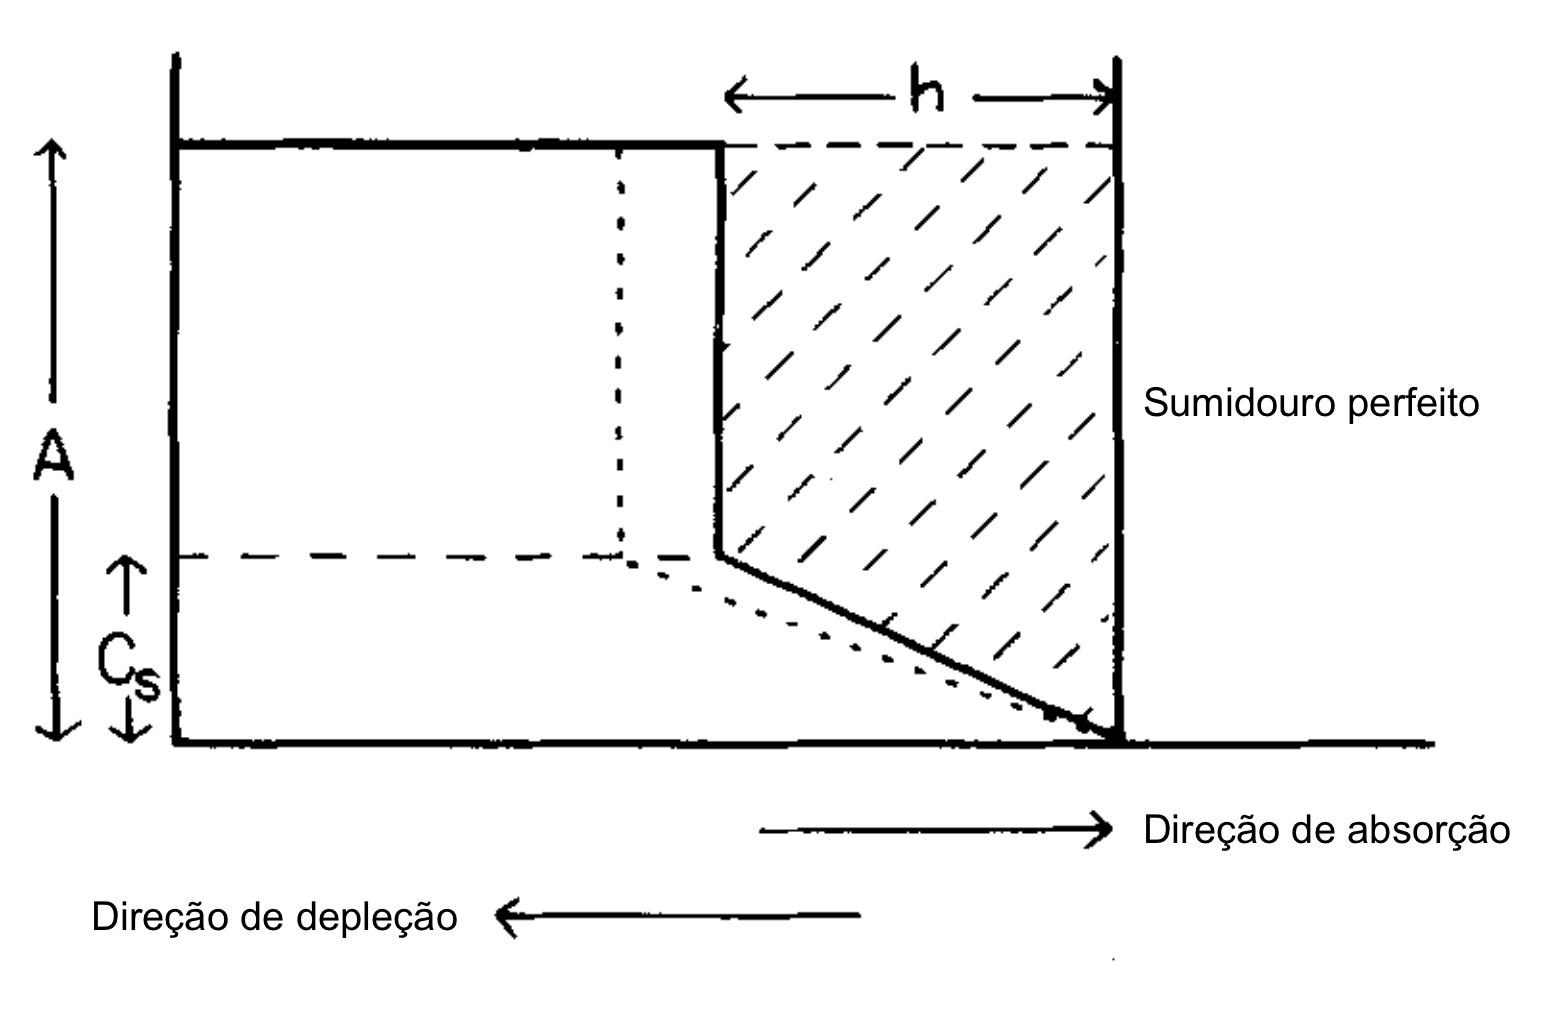
\includegraphics[width=0.6\textwidth]{figuras/Higuchi1961.png}
        \caption[Perfil de concentração teórica de uma matriz contendo fármaco em contato com um sumidouro perfeito]{Perfil de concentração teórica ao longo de uma matriz contendo fármaco em contato com um sumidouro perfeito (Higuchi, 1961).}
    \label{fig:Higuchi1961}
\end{figure}

Segundo Scheindlin (2004), em fármacos de liberação transdermal, um grande excesso de princípio ativo é colocado nos adesivos para manter o gradiente de concentração favorável à absorção. Assume-se aqui que esse seja o caso do etinilestradiol, extrapolando também para o anel vaginal. Sendo assim, pode ser observado que o perfil de difusão ao longo da camada polimérica do anel na região próxima da pele se assemelha à \Figura{fig:Higuchi1961}. Isso se deve à condição de contorno utilizada nessa borda, que assume a pele como um sumidouro perfeito devido a se tratar de uma mucosa. Na extremidade em contato com a solução, é possível perceber que a concentração não chega a zero, mas também não atinge o valor da concentração inicial. Isso é explicado pelo fato de ter sido estabelecida uma condição de fluxo zero em $x=0$, devido à consideração de que há uma quantidade finita de fármaco dentro do anel, e o fluxo ocorre em apenas uma direção.

Para o perfil de difusão ao longo da camada adesiva, é observado que apresenta, na extremidade $x = L$, um comportamento bem diferente da \Figura{fig:Higuchi1961}. Esse comportamento é esperado, considerando que o modelo foi desenvolvido considerando uma alta resistência nessa extremidade, criada pela pele. Essa condição é oposta à do sumidouro perfeito, portanto pode-se considerar que o modelo se adequa à realidade.

\section{Liberação de etinilestradiol ao longo do tempo}

\subsection{Liberação a partir do contraceptivo oral combinado}

A \Figura{fig:liberacao_coc} apresenta a concentração de etinilestradiol liberada a partir de uma pílula anticoncepcional no fluido gastrointestinal ao longo do tempo. É observado que a concentração de EE aumenta de forma contínua ao longo do tempo, atingindo um pico ao final do período de 24 horas. Ao se comparar com a referência da literatura para liberação de fármaco de primeira ordem, apresentada na \Figura{fig:primeira_ordem}, pode-se concluir que a curva obtida a partir do modelo apresenta o formato esperado, porém demora muito mais tempo para atingir os 80\% de liberação cumulativa do fármaco. Isso pode ser relacionado com os coeficientes $C_s$ e $k_d$ obtidos da literatura, ou com a própria natureza do COC de apresentar uma liberação controlada.

\begin{figure}[!htb]
    \centering
        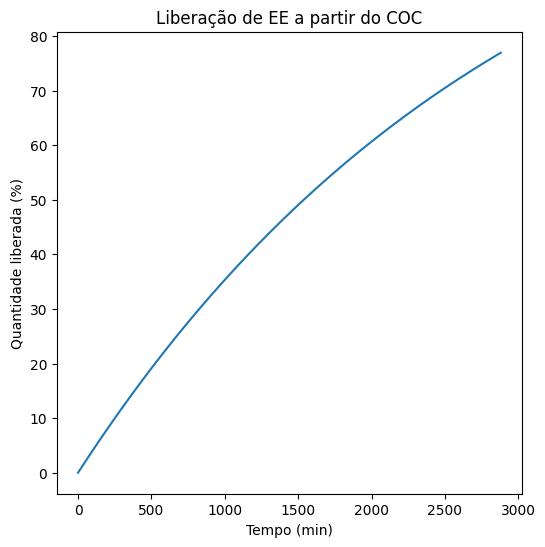
\includegraphics[width=0.46\textwidth]{figuras/liberacao_coc.png}
        \caption[Liberação cumulativa a partir do COC]{Quantidade de etinilestradiol (\%) liberada a partir do COC ao longo do tempo (min).}
    \label{fig:liberacao_coc}
\end{figure}

\begin{figure}[!htb]
    \centering
        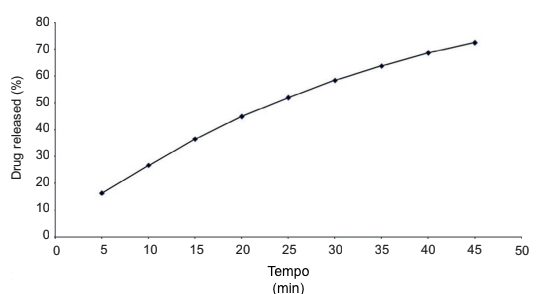
\includegraphics[width=0.6\textwidth]{figuras/primeira_ordem.png}
        \caption[Liberação de fármaco de primeira ordem]{Liberação de fármaco de primeira ordem: liberação cumulativa de fármaco (\%) versus tempo (min) (Bruschi, 2015).}
    \label{fig:primeira_ordem}
\end{figure}

\subsection{Taxa de liberação para cada matriz}

A fim de comparar as três diferentes matrizes estudadas entre si, foram plotadas as concentrações liberadas (\textmu g/mL) por tempo (dias) para cada uma delas, simulando a reposição no caso do COC e do adesivo, e abrangendo, assim, um período de 21 dias. O resultado é apresentado na \Figura{fig:liberacao_combinada}. Nela, podem ser observados picos regulares e decaimentos rápidos para a concentração liberada a partir do COC, uma liberação mais constante para o adesivo transdérmico e, por fim, uma liberação inicial rápida, seguida de uma estabilização em uma concentração mais baixa para o anel vaginal.

Esse gráfico pode ser comparado com a \Figura{fig:Heuvel}, obtida por Heuvel et. al (2005) a partir das concentrações plasmáticas das mulheres que participaram do estudo com cada um dos métodos contraceptivos. É perceptível que as concentrações obtidas na simulação foram muito mais altas do que as disponíveis na literatura, entretanto foi possível obter um perfil, no geral, muito similar para todas as matrizes estudadas.

\begin{figure}[!htb]
    \centering
        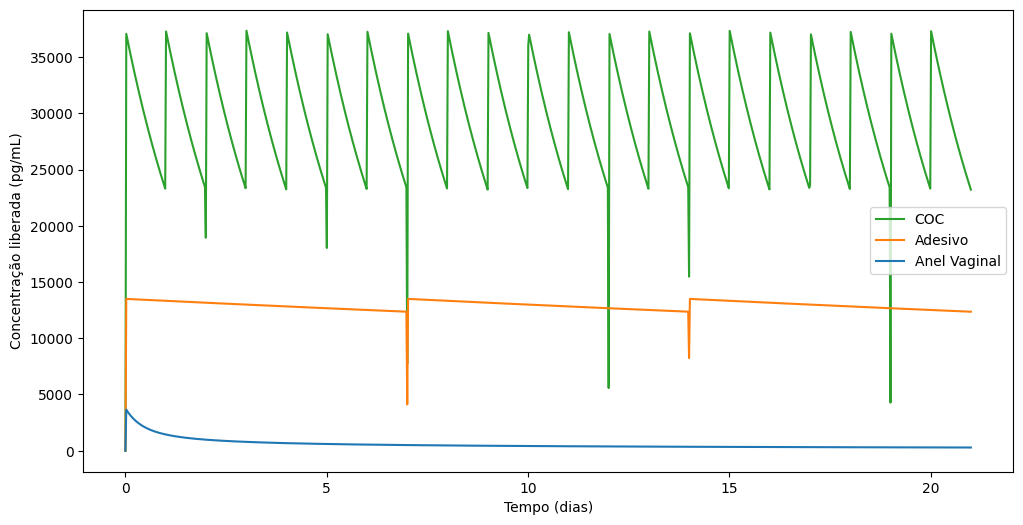
\includegraphics[width=1\textwidth]{figuras/liberacao_combinada.png}
        \caption[Liberação de etinilestradiol simulada ao longo do tempo]{Simulação da liberação de etinilestradiol (pg/mL) para o COC, adesivo e anel vaginal ao longo de 21 dias.}
    \label{fig:liberacao_combinada}
\end{figure}

\begin{figure}[!htb]
    \centering
        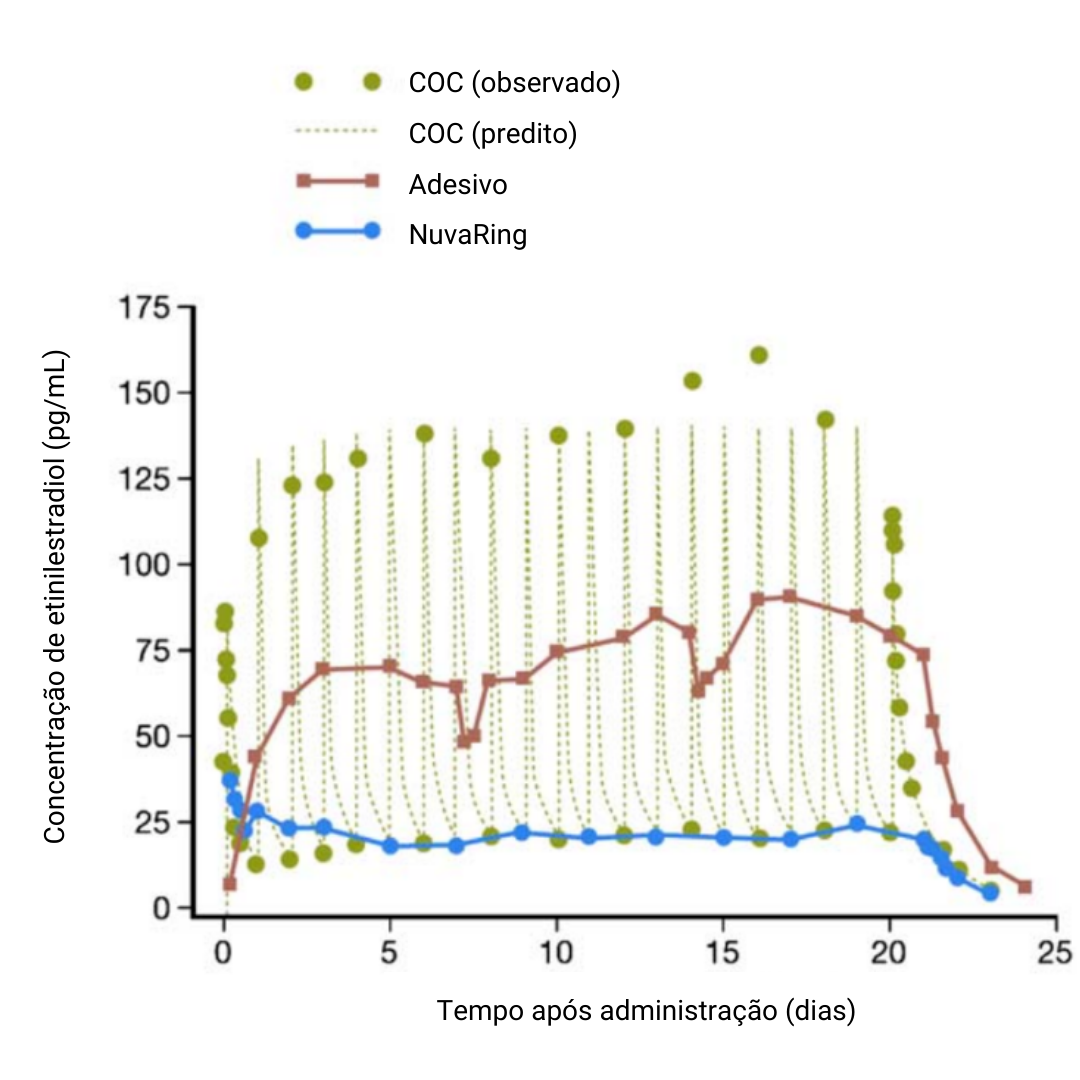
\includegraphics[width=0.68\textwidth]{figuras/Heuvel.png}
        \caption[Curvas experimentais de concentrações plasmáticas de EE]{Curvas obtidas a partir das concentrações plasmáticas de mulheres utilizando COC, adesivo e anel vaginal (Heuvel et. al, 2005)}
    \label{fig:Heuvel}
\end{figure}

A simulação realizada apresenta resultados coerentes com as afirmações da literatura de que a dosagem diária da pílula produz picos e vales na concentração de EE no sangue ao longo do tempo, enquanto o anel vaginal proporciona uma dosagem muito menor e mais estável (Heuvel et al. 2005). Além disso, observa-se que, de fato, a fim de compensar o metabolismo de primeira passagem, são liberadas concentrações mais elevadas do princípio ativo no COC do que nas demais matrizes (Kuhl, 2005). Corrobora-se também o fato de que o anel vaginal possui um efeito de liberação inicial rápida antes de atingir um estado estacionário na taxa de liberação, devido ao acúmulo de hormônios na superfície durante o armazenamento (Faundes, 2004).

A discrepância nos valores absolutos evidencia as limitações do modelo, advindas da desconsideração do metabolismo e eliminação do fármaco, fatores que provavelmente causam uma diminuição drástica nas concentrações plasmáticas. Dado que o objetivo principal desse trabalho diz respeito à modelagem da liberação de etinilestradiol, e não de sua concentração no sangue, essas limitações são aceitáveis dentro do escopo deste estudo. No entanto, para uma aplicação posterior, seria necessário integrar processos farmacocinéticos ao modelo, como metabolismo, distribuição, eliminação e absorção do fármaco. Além disso, ajustes nos parâmetros do modelo, como coeficientes de difusão e concentrações iniciais, com base em dados experimentais, poderiam melhorar a precisão das simulações e a aplicabilidade. 

\section{Análise de sensibilidade}

Os coeficientes de difusão nas matrizes poliméricas utilizados para os resultados apresentados foram selecionados com base nos valores das estimativas iniciais, mas multiplicados por fatores de conversão conforme o necessário, com o objetivo de obter resultados que permanecessem dentro da faixa esperada para a liberação do etinilestradiol nas matrizes analisadas. Essa abordagem permite uma análise preliminar da dinâmica de liberação, porém, sem uma precisão absoluta quanto aos valores dos coeficientes. Por isso, além da comparação com a literatura, foi realizada uma análise de sensibilidade com o intuito de demonstrar como variações nos coeficientes de difusão impactam cada uma das matrizes.

Para o adesivo transdérmico, o coeficiente de difusão que melhor se ajustou às condições físicas foi $D = 5,76 \times 10^{-13}$, isto é, 90000 vezes menor do que a estimativa original utilizada. Esse valor foi utilizado como base para a análise de sensibilidade realizada, comparando o perfil de difusão na extremidade em contato com a pele para $-50\% D$, $D$ e $+50\%D$. Os resultados estão dispostos na \Figura{fig:sensibilidade_adesivo}, onde pode ser observada uma maior diferença de concentração conforme se aumenta o valor de $D$. Assim, pode-se concluir que um valor maior de $D$ resulta em uma difusão mais rápida do 
fármaco, levando a uma diminuição mais rápida da concentração ao longo da espessura. Isso significa que, quanto menor o $D$, maior a resistência do meio à difusão, porém, uma variação pequena não produz resultados tão significativos. Esse fato pode explicar o motivo de ter sido necessário utilizar um valor tão mais baixo do que o inicial a fim de controlar melhor o perfil de liberação nessa matriz. É importante lembrar que não foi realizada uma simulação considerando a resistência da pele, então parte dessa resistência pode ter sido incorporada a esse modelo, levando a um $D$ mais baixo do que o da camada adesiva na realidade.

\begin{figure}[!htb]
    \centering
    \subfloat[$0,5D = 2,88 \times 10^{-13}$]{%
        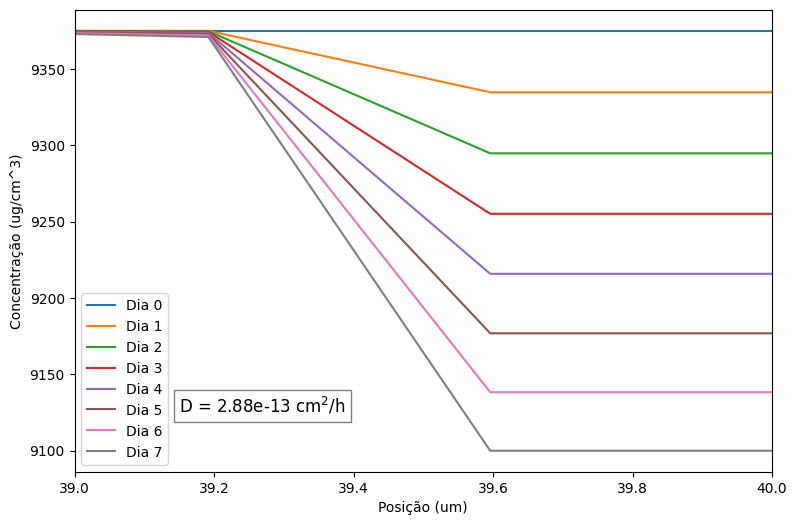
\includegraphics[width=0.65\textwidth]{figuras/sensibilidade_adesivo_05.png}%
        \label{fig:sensibilidade_adesivo_05}%
    }\\
    \subfloat[$D = 5,76 \times 10^{-13}$]{%
        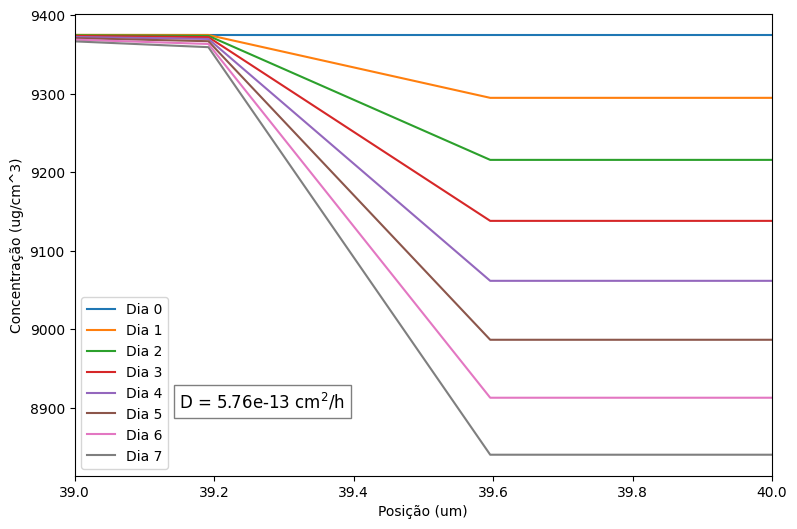
\includegraphics[width=0.65\textwidth]{figuras/sensibilidade_adesivo_1.png}%
        \label{fig:sensibilidade_adesivo_1}%
    }\\
    \subfloat[$1,5D = 8,64 \times 10^{-13}$]{%
        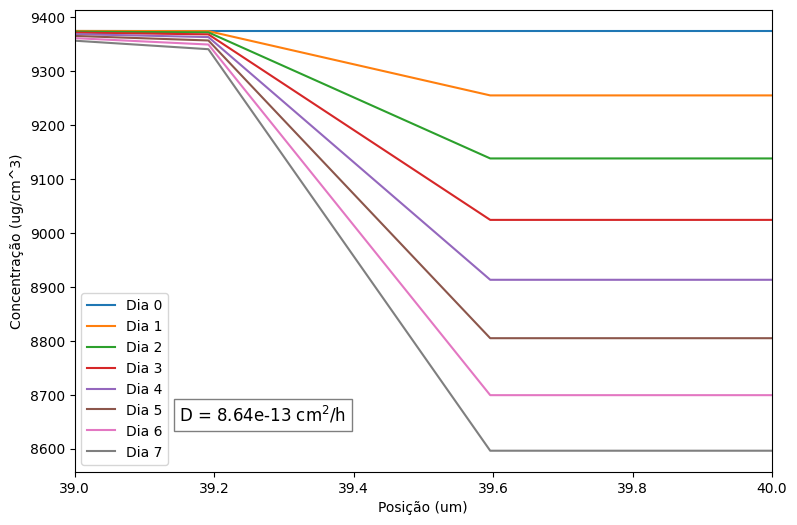
\includegraphics[width=0.65\textwidth]{figuras/sensibilidade_adesivo_50.png}%
        \label{fig:sensibilidade_adesivo_50}%
    }
    \caption[Análise de sensibilidade para o $D$ no adesivo transdérmico]{Análise de sensibilidade para o valor de $D$ no adesivo transdérmico, considerando \Subfigura{fig:sensibilidade_adesivo_05} -50\% $D$, \Subfigura{fig:sensibilidade_adesivo_1} $D$ e \Subfigura{fig:sensibilidade_adesivo_50} +50\% $D$}
    \label{fig:sensibilidade_adesivo}
\end{figure}

Para o anel vaginal, o coeficiente de difusão que melhor se ajustou às condições físicas foi $D = 7,92 \times 10^{-7}$, que é 5000 vezes menor do que o valor da estimativa inicial. Novamente, esse foi o valor foi utilizado como base para a análise de sensibilidade, comparando o perfil de difusão na extremidade em contato com a pele para $-50\% D$, $D$ e $+50\%D$. Os resultados estão dispostos na \Figura{fig:sensibilidade_anel}. Neles, pode ser novamente observada uma diminuição ligeiramente mais acentuada da concentração ao longo da posição quanto maior o valor de $D$, indicando menor resistência à difusão. O valor final bem maior do que o do adesivo, por si só, também corrobora o fato que se trata de um sistema com menor resistência, devido à aplicação ser em uma mucosa.

\begin{figure}[!htb]
    \centering
    \subfloat[$0,5D = 3,96 \times 10^{-7}$]{%
        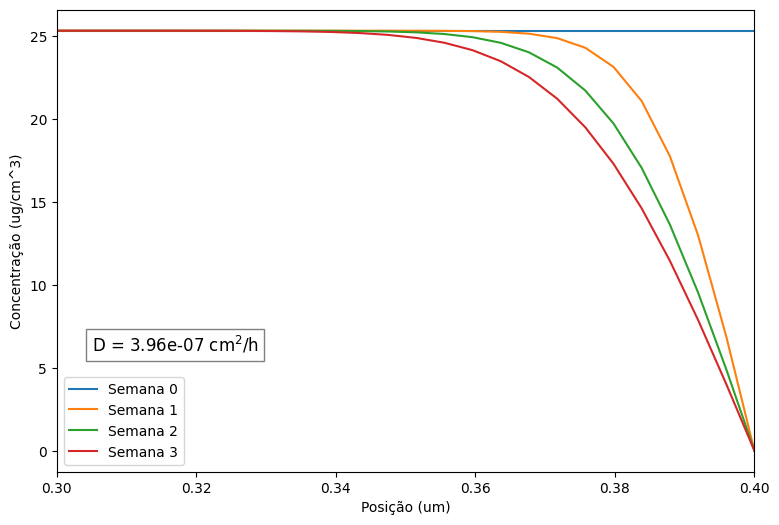
\includegraphics[width=0.62\textwidth]{figuras/sensibilidade_anel_05.png}%
        \label{fig:sensibilidade_anel_05}%
    }\\
    \subfloat[$D = 7,92 \times 10^{-7}$]{%
        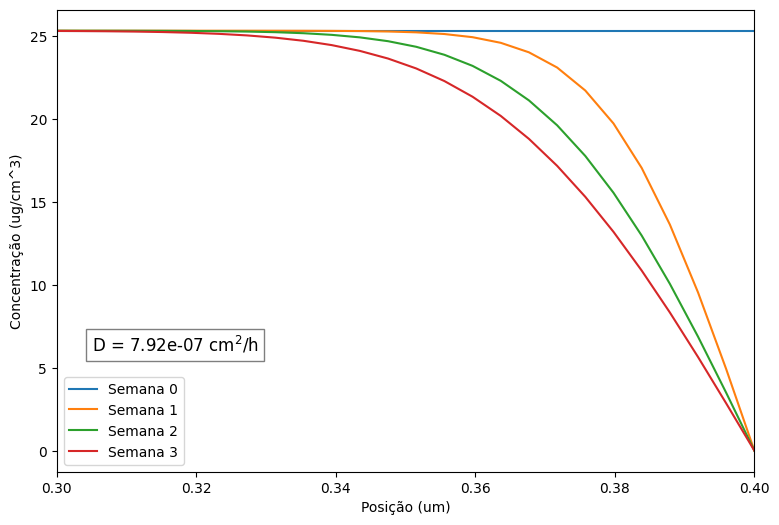
\includegraphics[width=0.62\textwidth]{figuras/sensibilidade_anel_1.png}%
        \label{fig:sensibilidade_anel_1}%
    }\\
    \subfloat[$1,5D = 1,19 \times 10^{-6}$]{%
        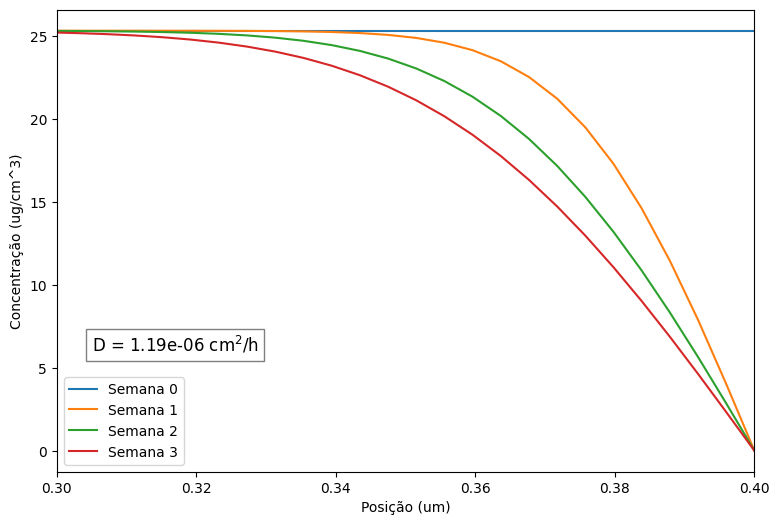
\includegraphics[width=0.62\textwidth]{figuras/sensibilidade_anel_50.png}%
        \label{fig:sensibilidade_anel_50}%
    }
    \caption[Análise de sensibilidade para o $D$ no anel vaginal]{Análise de sensibilidade para o valor de $D$ no anel vaginal, considerando \Subfigura{fig:sensibilidade_anel_05} -50\% $D$, \Subfigura{fig:sensibilidade_anel_1} $D$ e \Subfigura{fig:sensibilidade_anel_50} +50\% $D$}
    \label{fig:sensibilidade_anel}
\end{figure}

Por último, é importante ressaltar que já era esperado que os coeficientes de difusão para essas duas matrizes fossem menores do que os obtidos na literatura, afinal, ambos os valores eram para o $17\beta$-estradiol, que é uma molécula de raio menor, e portanto apresenta menos resistência à difusão. 
%%%%%%%%%%%%%%%%%%%%%%%%%%%%%%%%%%%%%%%%%%%%%%%%%%%%%%%%%%%%%%%%%%

%%%%%%%%%%%%%%%%%%%%%%%%%%%%%%%%%%%%%%%%%%%%%%%%%%%%%%%%%%%%%%%%%%
% O comando a seguir inclui o arquivo conclusoes.tex que contém o 
% capítulo de conclusões. 
%%%%%%%%%%%%%%%%%%%%%%%%%%%%%%%%%%%%%%%%%%%%%%%%%%%%%%%%%%%%%%%%%%
\chapter{Conclusão}\label{chp:conclusao}

Neste trabalho, foram desenvolvidos e analisados modelos computacionais para a liberação controlada de etinilestradiol em três diferentes matrizes: adesivo transdérmico, anel vaginal e contraceptivo oral combinado (COC). Utilizando a combinação de modelagem matemática, métodos numéricos e modelagem computacional, foi possível obter perfis de liberação que refletem as características específicas de cada sistema.

Para o adesivo transdérmico, foi observada uma liberação sustentada e gradual de etinilestradiol ao longo de sete dias, o que é ideal para manter níveis terapêuticos constantes no corpo. Este comportamento é consistente com a necessidade de fornecer uma dose constante ao longo do tempo, minimizando flutuações. Para o anel vaginal, foi identificada uma liberação inicial rápida seguida por uma estabilização em uma concentração mais baixa, um perfil muito similar com o descrito na literatura. Já para o contraceptivo oral combinado (COC), a liberação ao longo de 24 horas mostrou uma diminuição gradual e altas oscilações, refletindo a necessidade de administração diária para manter níveis terapêuticos. Este perfil é consistente com a prática de uso de contraceptivos orais.

Ao comparar os resultados das simulações com dados experimentais disponíveis na literatura, foi observado que as concentrações liberadas obtidas foram muito mais altas do que as relatadas na literatura para concentrações plasmáticas após administração. Essa discrepância pode ser atribuída ao fato de os modelos não levarem em consideração o metabolismo, a distribuição, a eliminação e a absorção do fármaco no corpo humano, nem a resistência da pele no modelo do adesivo transdérmico. Além disso, outra limitação é a questão dos coeficientes de difusão e parâmetros farmacocinéticos utilizados, que podem diferir dos valores reais, afetando a precisão dos resultados.

Em conclusão, este trabalho forneceu uma base inicial para a compreensão dos mecanismos de liberação e difusão de etinilestradiol em diferentes matrizes, as vantagens e limitações de cada um. De acordo com os resultados obtidos e com as informações da literatura, pode-se sugerir que haja o incentivo por parte das políticas públicas à consideração do adesivo transdérmico e do anel vaginal como métodos contraceptivos alternativos à pílula anticoncepcional. Esses métodos, apesar de mais caros, liberam o hormônio em níveis mais baixos e mais estáveis, sendo boas opções para mulheres que não se adaptarem à dosagem diária ou aos efeitos colaterais da pílula. 

A integração de processos metabólicos e ajustes nos parâmetros do presente modelo são importantes para aprimorar a precisão e a aplicabilidade dos resultados, contribuindo para o desenvolvimento de métodos contraceptivos mais eficazes e seguros.
%%%%%%%%%%%%%%%%%%%%%%%%%%%%%%%%%%%%%%%%%%%%%%%%%%%%%%%%%%%%%%%%%%

% Comandos para incluir as referências bibliográficas
% Define espaçamento simples em cada referência
\begin{singlespacing}

% Adiciona uma linha em branco entre duas referências
\setlength\bibitemsep{10pt}   
%
% Adiciona as referências bibliográficas.
\nocite{*}
\printbibliography[heading=bibintoc, title={Referências bibliográficas}]
\end{singlespacing}

%%%%%%%%%%%%%%%%%%%%%%%%%%%%%%%%%%%%%%%%%%%%%%%%%%%%%%%%%%%%%%%%%%
% Os anexos, se houver, vêm depois das referências:
%%%%%%%%%%%%%%%%%%%%%%%%%%%%%%%%%%%%%%%%%%%%%%%%%%%%%%%%%%%%%%%%%%
\appendix
%%%%%%%%%%%%%%%%%%%%%%%%%%%%%%%%%%%%%%%%%%%%%%%%%%%%%%%%%%%%%%%%%%

%%%%%%%%%%%%%%%%%%%%%%%%%%%%%%%%%%%%%%%%%%%%%%%%%%%%%%%%%%%%%%%%%%
% Os comandos a seguir incluem os arquivos de capítulos do 
% apêndice. Observe o comando \appendix na linha anterior.
%%%%%%%%%%%%%%%%%%%%%%%%%%%%%%%%%%%%%%%%%%%%%%%%%%%%%%%%%%%%%%%%%%
% OBS: Comente as linhas a seguir (ou delete-as) se não houver um 
% apêndice
%%%%%%%%%%%%%%%%%%%%%%%%%%%%%%%%%%%%%%%%%%%%%%%%%%%%%%%%%%%%%%%%%%

\chapter{Código desenvolvido}

\section{Modelagem para a difusão no adesivo transdérmico}
\begin{verbatim}
import numpy as np
import matplotlib.pyplot as plt
import pandas as pd
from scipy.sparse import diags
from scipy.sparse.linalg import spsolve

# Dados
L1 = 0.004  # Espessura da matriz (cm)
D1 = 0.0000005184 / 900000  # Coeficiente de difusão (cm^2/h)
C10 = 9375  # Concentração inicial de EE (ug/cm^3)
Km = 1  # Coeficiente de partição matriz-pele (s.u.)
V1 = 0.08  # Volume total do adesivo (cm³)

# Número de pontos
Nx1 = 100  # Número de pontos espaciais

# Variáveis
T1 = 168  # Tempo total coberto na simulação (h)
dx1 = L1 / Nx1  # Passo espacial

# Passo temporal
dt = 0.1

# Concentrações iniciais
C1 = np.zeros((Nx1, int(T1/dt) + 1))
C1[:, 0] = C10

# Quantidade total de fármaco disponível no adesivo
total_farmaco_disponivel_adesivo = C10 * V1

# Coeficientes para o método de Crank-Nicolson
alpha1 = D1 * dt / (2 * dx1**2)

# Matrizes tridiagonais
A1 = diags([-alpha1, 1 + 2*alpha1, -alpha1], [-1, 0, 1], \
            shape=(Nx1-2, Nx1-2))
A1 = A1.tocsc()  # Conversão para o formato CSC
B1 = diags([alpha1, 1 - 2*alpha1, alpha1], [-1, 0, 1], \
            shape=(Nx1-2, Nx1-2))

# Método de Crank-Nicolson
total_released = 0
for n in range(0, int(T1/dt)):

    # Resolver para C1
    b1 = B1 @ C1[1:-1, n]
    C1[1:-1, n + 1] = spsolve(A1, b1)
    
    # Condição de contorno de fluxo zero para x=0
    C1[0, n + 1] = C1[1, n + 1]

    # Condição de contorno utilizando o coeficiente 
    # de partição para x=L1
    C1[-1, n + 1] = Km * C1[-2, n + 1]

    # Calcular a quantidade total de fármaco liberado a cada dia
    if (n + 1) % int(24/dt) == 0:
        daily_released = np.sum(C1[:, n + 1] - \
                        C1[:, n + 1 - int(24/dt)]) * dx1
        if daily_released > 20:
            # Parar a liberação de fármaco para o restante do dia
            C1[:, n + 1] = C1[:, n + 1 - int(24/dt)]
        total_released += daily_released

        # Verificar se a quantidade total de fármaco liberado 
        # ultrapassa a quantidade disponível
        if total_released > total_farmaco_disponivel_adesivo:
            print("A quantidade total de fármaco liberado" 
                "ultrapassa a quantidade disponível no adesivo.")
            C1[:, n + 1:] = 0
            break

# Converter tempo para dias
time_days = np.linspace(0, 7, int(T1/dt) + 1)

# Conversão de cm para µm
space_um_vehicle = np.linspace(0, L1 * 1e4, Nx1)

# Selecionar pontos temporais específicos para exibir na tabela
time_points = [int(24/dt * day) for day in range(0, 8)]
time_labels = [f't={day:.2f} dias' for day in range(0, 8)]

# Criar DataFrames para armazenar os resultados
results_vehicle = pd.DataFrame(C1[:, time_points], \
                                columns=time_labels)
results_vehicle.index = np.linspace(0, L1, Nx1)

# Exibir as tabelas
from IPython.display import display
print(
    "Perfis de Concentração na Camada Adesiva em Pontos" 
    "Temporais Selecionados:")
display(results_vehicle)

# Plotar o perfil de difusão na matriz
from mpl_toolkits.axes_grid1.inset_locator import inset_axes

# Plot principal
fig, ax = plt.subplots(figsize=(14, 8))
for i, n in enumerate(time_points):
    ax.plot(space_um_vehicle, C1[:, n], \
            label=f'Dia {int(time_days[n])}')

# Configurações do plot principal
ax.set_xlabel('Posição (µm)')
ax.set_ylabel('Concentração (µg/cm³)')
ax.legend()
ax.set_title('Difusão de EE na Camada Adesiva')

# Plot com zoom
axins = inset_axes(ax, width="40%", height="40%", \
                    loc="upper right")
for i, n in enumerate(time_points):
    axins.plot(space_um_vehicle, C1[:, n])

# Definindo os limites da região ampliada
x1, x2 = 0, 1
y1, y2 = 8800, 9400
axins.set_xlim(x1, x2)
axins.set_ylim(y1, y2)

plt.show()
\end{verbatim}

\section{Modelagem para a difusão no anel vaginal}
\begin{verbatim}
import numpy as np
import matplotlib.pyplot as plt
import pandas as pd
from scipy.sparse import diags
from scipy.sparse.linalg import spsolve

# Dados
L2 = 0.4  # Espessura da matriz (cm)
D2 = 0.00000792/10 # Coeficiente de difusão na matriz (cm^2/h)
C20 = 25.33 # Concentração inicial de EE na matriz (ug/cm^3)
V2 = 106.58  # Volume total do adesivo (cm³)

# Número de pontos
Nx2 = 100  # Número de pontos espaciais na matriz

# Variáveis
T2 = 504  # Tempo total coberto na simulação (h)
dx2 = L2 / Nx2  # Passo espacial para a matriz

# Passo temporal
dt2 = 0.1

# Concentrações iniciais
C2 = np.zeros((Nx2, int(T2/dt2) + 1))
C2[:, 0] = C20

# Quantidade total de fármaco disponível no anel
total_farmaco_disponivel_anel = C20 * V2

# Coeficientes para o método de Crank-Nicolson
alpha = D2 * dt2 / (2 * dx2**2)

# Matrizes tridiagonais
A2 = diags([-alpha, 1 + 2*alpha, -alpha], [-1, 0, 1], \
        shape=(Nx2-2, Nx2-2))
A2 = A2.tocsc()
B2 = diags([alpha, 1 - 2*alpha, alpha], [-1, 0, 1], \
        shape=(Nx2-2, Nx2-2))

# Método de Crank-Nicolson
for n in range(0, int(T2/dt2)):
    if n % 100 == 0:
        print(f"Iteração {n} de {int(T2/dt2)}")
    # Resolver para C
    b2 = B2 @ C2[1:-1, n]
    C2[1:-1, n + 1] = spsolve(A2, b2)

    # Condição de contorno de fluxo zero para x=0
    C2[0, n + 1] = C2[1, n + 1]

    # Condição de contorno para x=L
    C2[-1, n + 1] = 0

    # Calcular a quantidade total de fármaco liberado a cada dia
    if (n + 1) % int(24/dt) == 0:
        daily_released = np.sum(C2[:, n + 1] - \
                        C2[:, n + 1 - int(24/dt)]) * dx2
        if daily_released > 15:
            # Parar a liberação de fármaco para o restante do dia
            C2[:, n + 1] = C2[:, n + 1 - int(24/dt)]
        total_released += daily_released

        # Verificar se a quantidade total de fármaco liberado 
        # ultrapassa a quantidade disponível
        if total_released > total_farmaco_disponivel_anel:
            print("A quantidade total de fármaco liberado" 
                "ultrapassa a quantidade disponível no anel.")
            C2[:, n + 1:] = 0
            break

# Converter tempo para semanas
num_weeks = T2 // (24 * 7)
time_weeks = np.linspace(0, num_weeks, int(T2/dt2) + 1)

# Selecionar pontos temporais específicos para exibir na tabela
time_points = [int((7 * 24) / dt2) * \
            week for week in range(num_weeks + 1)]
time_labels = [f'Semana {week}' for week in range(num_weeks + 1)]

# Criar DataFrames para armazenar os resultados
results_vehicle = pd.DataFrame(C2[:, time_points], \
                        columns=time_labels)
results_vehicle.index = np.linspace(0, L2, Nx2)

# Exibir as tabelas
from IPython.display import display
print("Perfis de Concentração na Camada Polimérica" 
    "em Pontos Temporais Selecionados:")
display(results_vehicle)

# Plotar o perfil de difusão
plt.figure(figsize=(12, 6))
for tp in time_points:
    plt.plot(np.linspace(0, L2, Nx2), C2[:, tp], \
            label=f'{time_labels[time_points.index(tp)]}')
plt.xlabel('Posição (cm)')
plt.ylabel('Concentração (ug/cm^3)')
plt.legend()
plt.title('Difusão de EE na Camada Polimérica')
plt.show()
\end{verbatim}

\section{Modelagem para a liberação a partir do COC}
\begin{verbatim}
import numpy as np
import matplotlib.pyplot as plt

# Dados
Cs = 18.7  # Solubilidade máxima do EE no fluido gastrointestinal (ug/cm^3)
kd = 0.02  # Constante de dissolução (1/h)
T3 = 24  # Tempo total coberto na simulação (h)
dt = 0.1  # Passo temporal (h)
C_max = 15  # Concentração máxima permitida (ug/cm^3)

# Função que representa a EDO
def dCdt(Cd, t):
    return kd * (Cs - Cd)

# Inicialização
t_values = np.arange(0, T3 + dt, dt)
C3 = np.zeros(len(t_values))
C3[0] = 0  # Concentração inicial de EE no fluido gastrointestinal

# Método de Runge-Kutta de quarta ordem (RK4) com limite de concentração
for i in range(1, len(t_values)):
    t = t_values[i-1]
    Cd = C3[i-1]

    k1 = dt * dCdt(Cd, t)
    k2 = dt * dCdt(Cd + 0.5 * k1, t + 0.5 * dt)
    k3 = dt * dCdt(Cd + 0.5 * k2, t + 0.5 * dt)
    k4 = dt * dCdt(Cd + k3, t + dt)

    # Calcular a nova concentração e impor o limite
    C3[i] = Cd + (k1 + 2*k2 + 2*k3 + k4) / 6
    if C3[i] > C_max:
        C3[i] = C_max

# Plotar os resultados
plt.figure(figsize=(12, 6))
plt.plot(t_values, C3, label='Concentração liberada')
plt.xlabel('Tempo (h)')
plt.ylabel('Concentração (ug/cm^3)')
plt.legend()
plt.title('Liberação de EE a partir da Pílula')
plt.show()
\end{verbatim}

\section{Concentração liberada em função do tempo para cada matriz}

\begin{verbatim}
import numpy as np
import matplotlib.pyplot as plt

# Cálulo das taxas para cada matriz

def calculate_release_rate(C, dx=None):
    release_rate = np.zeros(C.shape[1]) if C.ndim == 2 else \
                    np.zeros(len(C))
    for n in range(1, C.shape[1] if C.ndim == 2 else len(C)):
        if C.ndim == 2: # Adesivo e anel
            # Usar a média da concentração ao longo da matriz 
            # para cada ponto temporal
            avg_concentration = np.mean(C[:, n] - C[:, n - 1])
            rate = avg_concentration
        else: # COC
            dC = C[n] - C[n - 1]
            rate = dC
        release_rate[n] = rate
    return np.abs(release_rate)

# Calculando a taxa
release_rate_patch = calculate_release_rate(C1, dx1)
release_rate_ring = calculate_release_rate(C2, dx2)
release_rate_pill = calculate_release_rate(C3)

# Criando subplots para plotar cada matriz separadamente
fig, axs = plt.subplots(1, 3, figsize=(18, 6))

# Plotando resultados para o adesivo
axs[0].plot(np.linspace(0, T1, len(release_rate_patch)), \
            release_rate_patch, label='Taxa de Liberação - Adesivo')
axs[0].set_xlabel('Tempo (h)')
axs[0].set_ylabel('Taxa de Liberação (ug/mL)')
axs[0].set_title('Adesivo Transdérmico')
axs[0].legend()

# Plotando resultados para o anel vaginal
axs[1].plot(np.linspace(0, T2, len(release_rate_ring)), \
            release_rate_ring, label='Taxa de Liberação - Anel')
axs[1].set_xlabel('Tempo (h)')
axs[1].set_ylabel('Taxa de Liberação (ug/mL)')
axs[1].set_title('Anel Vaginal')
axs[1].set_xlim(0, 1)  # Recorte de tempo para a primeira hora
axs[1].legend()

# Plotando resultados para o COC
axs[2].plot(np.linspace(0, T3, len(release_rate_pill)), \
            release_rate_pill, label='Taxa de Liberação - COC')
axs[2].set_xlabel('Tempo (h)')
axs[2].set_ylabel('Taxa de Liberação (ug/mL)')
axs[2].set_title('Comprimido Oral Combinado')
axs[2].legend()

# Adicionar título unificado
fig.suptitle('Taxa de Liberação de Etinilestradiol', fontsize=16)

# Ajustar layout
plt.tight_layout()
plt.show()

# Plotando as matrizes juntas e simulando reposição

# Parâmetros
dt = 0.1  # Passo temporal (h)
T_total = 21 * 24  # Tempo total de 21 dias em horas
num_days = 21  # Número total de dias

# Função para empilhar as curvas simulando a reposição
def stack_curves(data, repeat_interval, total_time, dt):
    num_repeats = int(total_time / repeat_interval)
    stacked_data = np.zeros(int(total_time / dt))
    for i in range(num_repeats):
        start_idx = int(i * repeat_interval / dt)
        end_idx = start_idx + len(data)
        stacked_data[start_idx:end_idx] = data
    return stacked_data

# Empilhar as curvas
release_rate_pill_stacked = \
    stack_curves(release_rate_pill[:int(24/dt)],24, T_total, dt)
release_rate_patch_stacked = \
    stack_curves(release_rate_patch[:int(168/dt)], 168, T_total, dt)
release_rate_ring_stacked = \
    stack_curves(release_rate_ring[:int(504/dt)], 504, T_total, dt)

# Convertendo as taxas de liberação de µg/h para pg/h
release_rate_pill_stacked *= 1e6
release_rate_patch_stacked *= 1e6
release_rate_ring_stacked *= 1e6

# Redução do número de pontos no eixo x 
# para evitar erro de tamanho da imagem
num_points = 1000
x_values = np.linspace(0, num_days, num_points)
release_rate_pill_reduced = np.interp(x_values, \
    np.linspace(0, num_days, len(release_rate_pill_stacked)), \
    release_rate_pill_stacked)
release_rate_patch_reduced = np.interp(x_values, \
    np.linspace(0, num_days, len(release_rate_patch_stacked)), \
    release_rate_patch_stacked)
release_rate_ring_reduced = np.interp(x_values, np.linspace(0, num_days, \
len(release_rate_ring_stacked)), release_rate_ring_stacked)

# Definindo cores personalizadas
color_ring = '#1f77b4'
color_patch = '#ff7f0e'
color_pill = '#2ca02c'

# Plotar os resultados
plt.figure(figsize=(12, 6))
plt.plot(x_values, release_rate_pill_reduced, label='COC', color=color_pill)
plt.plot(x_values, release_rate_patch_reduced, label='Adesivo', \
            color=color_patch)
plt.plot(x_values, release_rate_ring_reduced, label='Anel Vaginal', \
            color=color_ring)
plt.xlabel('Tempo (dias)')
plt.ylabel('Concentração liberada (pg/h)')
plt.title('Liberação de etinilestradiol ao longo do tempo')
plt.legend()
plt.show()
\end{verbatim}

\end{document}